\documentclass[twoside, english, notitlepage, 12pt]{uiofysmaster}

\usepackage{miscellaneous/packages/packages}
\pgfplotsset{compat=newest} %compatibility

\addbibresource{miscellaneous/references.bib}

\author{Oliver Lerstøl Hebnes}
\title{Predicting\\
solid-state qubit\\
material host
}
\date{\today}

\begin{document}
\hypersetup{pageanchor=false}
\frontmatter
    \maketitle

    %\begin{abstract}
    %Recent developments of high-throughput databases has shown encouraging results for novel materials discovery. %Here,
%Recent applications of machine learning for novel materials discovery have shown encouraging results in dealing with the large data
In this thesis,
we perform an exploratory analysis for finding novel material hosts to be used in quantum technology. We have developed data extraction tools for numerous databases, and constructed over $4800$ physics-informed features for a dataset consisting of more than $25000$ materials.
Furthermore, we have developed and implemented three data mining approaches, termed \textit{the Ferrenti approach}, \textit{the augmented Ferrenti approach} and \textit{the insightful approach} for defining three distinct training sets for the supervised machine learning algorithms logistic regression, decision tree, random forest and gradient boost to be trained on.

We find a lack of consistent results for the Ferrenti approach and the augmented Ferrenti approach due to a too broad formulation of the training set, whereas the restrictions set in the insightful approach proved suitable. All models agreed on $214$ predicted candidates, with examples such as ZnGeP$_2$, MgSe, BP, BC$_2$N, BP, Ge, GeC, InP and InAs. All approaches and all models agreed on a subset of $47$ eligible candidates of $8$ elemental, $29$ binary and $10$ tertiary compounds.

% We suggest the $28$ materials as the most promising novel qubit material hosts candidates present in our dataset.

    %\end{abstract}

    %\begin{acknowledgements}
    %%No one could have ever imagined how the last year would turn out to be. Essential keywords include quaranteene, isolation and social distancing. Consequently, I believe this puts bits and pieces more easily in perspective since we are able to spend more time with ourself and our own thoughts. Therefore, I truly have many persons to thank for pulling me through this thesis.

The dream of having a social life during my masters was utterly shattered by the ongoing covid-19 pandemic. I recall joking ``see you after easter'' when the University locked down two weeks before easter the year $2020$. Now, $60$ weeks later, I'm still waiting for the reunion.
I was not certain that I would come out on the other side with a degree at all. For that, I truly have many persons to thank for pulling me through.

I'd like to thank my main supervisor, Morten, for being such an inspiring role model. I did not fancy studying until I encountered your positive energy and pure pleasure of research.


Secondly, I would like to thank my supervisors Marianne, Øyvind, Sebastian and Lasse for excellent counseling through both fun and difficult times. Thank you for shining light upon my path and letting me know when my good ideas were bad and bad ideas were good (mostly just bad).

% For this, I owe a thanks to the great people of MENA and computational science group.

Thirdly, I would like to thank the people that made the years of studying the best so far. Thank you, Mohamed, Jens, Erik, Jørn, Andreas, and the rest of the people at MENA and CS for sharing obligs, discussions, early mornings, late evenings, lunch breaks, pump-sundays at Athletica, hangovers, cabin trips, and occasional nonsense.

I would also like to thank my family's moral support and encouragement even though I am positive that they had no idea what I was talking about.


%Pre-corona, I had no idea that the years of attending the University of Oslo would be the best years I've had so far. In particular, I've shared many obligs, discussions, early mornings, late evenings, pump-sundays at Athletica, hangovers, cabin trips, and occasional nonsense with Mohamed, Jens, Erik, Jørn, Andreas, and the rest of the people at MENA.

Last but not least, I would like to thank my girlfriend Hanna for limitless support throughout this journey and for sacrificing a dining table so I could have a place to study. I may have written a thesis, but I believe you have \emph{suffered} a thesis.

    %\end{acknowledgements}

    \setcounter{tocdepth}{2}
    \tableofcontents
    %\listoffigures
    %\newpage

\mainmatter
    %\part{Introduction}
      %\chapter{Introduction}

This it The introduction.
Another coffee.

Trengs det egentlig undertitler her? Tenketenketenk
\newpage
\section{Motivation}
\section{Holy grail}
\section{Structure of thesis}


    %\part{Theory}
        %\chapter{Semiconductor quantum platforms}

This chapter will provide a brief overview of the current state-of-the-art in quantum technological advances. This will not only give us insights in how the technology is being used today, but also grant us the opportunity to discuss key concepts that are fundamental to understand for this thesis. Thereafter we will look into how materials are built up, and what the characteristics of a semiconductor is.
%Importantly, it will motivate the reasoning for finding new materials that can be used in devices for this purpose.

\section{Quantum technologies}

\textit{Quantum technology} (QT) refers to practical applications and devices that utilize the principles of quantum physics as a foundation. Technologies in this spectrum are based on concepts such as \textit{superposition}, \textit{entanglement} and \textit{coherence}, which are all closely related to one another.

A quantum superposition refers to that any two or more quantum eigenstates can be added together into another valid quantum state, such that every quantum state can be represented as a sum, or a superposition, of two or more distinct states. This is according to the wave-particle duality which states that every particle or another quantum entity may be described as either a particle or a wave. When measuring the state of a system residing in a superposition of eigenstates, however, the system falls back to one of the basis states that formed the superposition, destroying the original configuration.

Quantum entanglement refers to when a two- or many-particle state cannot be expressed independently of the state of the other particles, even when the particles are separated by a significant distance. As a result, the many-particle state is termed an entangled state \cite{Griffiths2017}.

Quantum coherence arises if two waves coherently interfere with each other and generate a superposition of the two states with a phase relation. Likewise, loss of coherence is known as \textit{decoherence}.

%The terms superposition, entanglement and coherence are closely related. The two latter terms are the primary features of quantum mechanics that are lacking in classical mechanics, giving rise to paradoxes such as Einstein's famous Schrödingers cat, which is both dead and alive at the same time when in its coherent state inside a closed box.

Another concept that the reader should be familiar with is the famous Heisenberg uncertainty principle. It states that
\begin{align}
    \sigma_x \sigma_p \leq \frac{\hslash}{2},
    \label{eq:uncertainty}
\end{align}
where $\sigma_x$ is the standard deviation for the position and $\sigma_p$ is the standard deviation in momentum. This means that we cannot accurately predict both the position and momentum of a particle at the same time. Thus, we often calculate the probability for a particle to be in a state which results in concepts such as an electron sky surrounding an atom core. However, remember that equation (\ref{eq:uncertainty}) is an inequality, which means that it is possible to create a state where neither the position nor the momentum is well defined.

\subsection{Quantum computation}
%The evolution of the digital worlds computational powers is a remarkable piece of history
The start of the digital world's computational powers can be credited to Alan Turing. In 1937, Turing \cite{Turing1937} published a paper where he described the \textit{Turing machine}, which is regarded as the foundation of computation and computer science. It states that only the simplest form of calculus, such as boolean Algebra ($1$ for true and $0$ for false), is actually computable. This required developing hardware that could handle classical logic operations, and was the basis of transistors that are either in the state ON or OFF depending on the electrical signal. Equipped with a circuit consisting of wires and transistors, commonly known as a computer, we could develop software to solve all kinds of possible applications.

Driven by the development of software, conventional computers have in accordance to Moore's law \cite{Moore1965}, doubled the amount of transistors on integrated circuit chips every two years as a result of smaller transistors. Furthermore, the clock frequency has enhanced with time, resulting in a doubling of computer performance every 18 months \cite{Pavicic2006}. Alas, miniaturization cannot go on forever as transistors are mass-produced at $5$ nm today and are expected to reach a critical limit of $3$ nm in the following years \cite{Gwennap2020}.

To sustain the digital world's increasing computational demand, other alternatives than the conventional classical computer must be explored. This is where quantum computation comes into the picture. The term quantum computer is a device that exploits quantum properties to solve certain computational problems more efficiently than allowed by Boolean logic \cite{Weber2010}.

The idea is to pass information in the form of a quantum bit, or \textit{qubit} for short. They are the building blocks of quantum computers, and as opposed to the conventional $0$ or $1$-bits that classical computers are based on, they can inhabit any superposition of the states $0$ or $1$. This is illustrated in figure \ref{fig:qubit and bit}.

%Since a qubit has a quantum nature and is the counterpart to the classical bit, it naturally follows that it is in the center of attention in quantum computation\footnote{There exists other systems such as the quantum d-state system, known as \textit{qudits}, that can also be utilised in quantum computation \cite{Ladd2010}.}.

The architecture of a gate-based quantum computer is dependent on a set of quantum logic gates that perform unitary transformations on sets of qubits \cite{DiVincenzo2000, Ladd2010}. Other implementations of quantum computers exists, such as the adiabatic quantum computer. This approach is not based on gates, but on defining the answer of a problem as the ground state of a complex network of interactions between qubits, and then controlling the interactions to adiabatically evolve the system to the ground state \cite{Mizel2007}.

\begin{wrapfigure}{r}{0.5\textwidth}
  \centering
  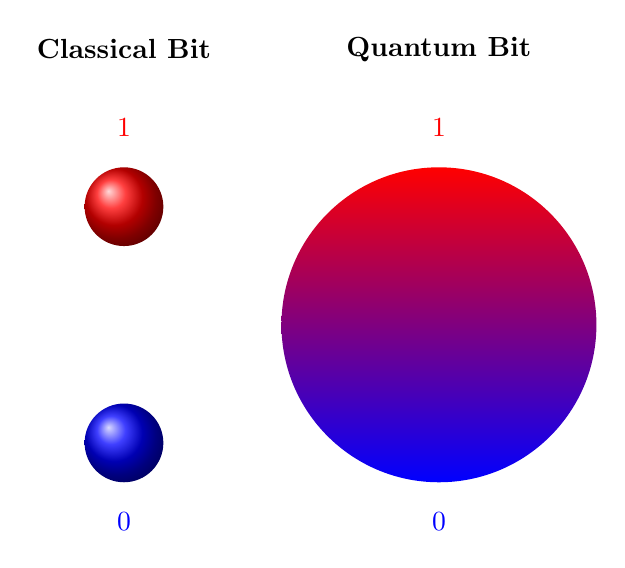
\begin{tikzpicture}[scale=1]
    \node[font=\bfseries] at (0,2) {Classical Bit};
    \node[font=\bfseries] at (4,2) {Quantum Bit};

    \node[color=red] at (0,1) {$1$};
    \node[color=blue] at (0,-4) {$0$};

    \node[shade,shading=ball,circle,ball color=blue,minimum size=1cm] (ball) at (0,-3) {};
    \node[shade,shading=ball,circle,ball color=red,minimum size=1cm] (ball) at (0,0) {};

    \node[color=red] at (4,1) {$1$};
    \node[color=blue] at (4,-4) {$0$};
    \node[shade, shading=ball,circle,top color=red, bottom color=blue, minimum size=4cm] (ball) at (4,-1.5) {};
  \end{tikzpicture}
  \caption{Conceptual illustration of the two-level classical bit, which are restricted to the boolean states 1 (true) or 0 (false), and the quantum bit that can be in any superposition of the states 0 or 1.}
  \label{fig:qubit and bit}
\end{wrapfigure}


It has been demonstrated that exponentially complex problems can be reduced to polynomially complex problems for quantum computers \cite{Pavicic2006}. For example, a quantum search algorithm found by Grover \cite{Grover1997} offers a quadratic speed-up compared to classical algorithms, while Shor's quantum integer factorization algorithm \cite{Shor1994} presents an exponential speed-up. Intriguingly, Google reported in $2019$ that they ran a random number generator algorithm on a superconducting processor containing 53 qubits in $200$ seconds, which would most likely take several times longer for a classical supercomputer to solve \cite{Martinis2019}. It is anticipated that quantum computers will excel in exceedingly complex problems, while many simpler tasks may not see any speed-up at all compared to the classical regime. Hence, quantum- and classical computers are envisioned to coexist for each their purpose.

%However, it is not to avoid that both quantum  hardware and -software is in its preliminary phase of development, and it will be interesting to follow up the progression the following years.

Quantum computing is a highly sought-after goal, but there are extensive challenges that needs to be adressed. Controlling a complex many-qubit system is difficult, since it is not always possible to establish interactions between qubits \cite{DiVincenzo2000} and maintain entaglement over both time and distance. Additionally, decoherence and other quantum noise occurs as a result of the high volatility of quantum states, making quantum state manipulation prone to errors. The \textit{quantum error correction} protocols and the theory of \textit{threshold theorem} deals with this vulnerability, stating that noise most likely does not pose any fundamental barrier to the performance of large-scale computations \cite{Pavicic2006}.

%Quantum hardware and -software are both in the preliminary stage of development, and it will be interesting to follow their progress the following years.

\subsection{Quantum computing requirements}
As ever-promising the concepts of quantum technology are, the physical realizations are in the preliminary stage of development. Here we will concretize critical principles for a physical realisation of a quantum platform.

\begin{quote}
   ``I always said that in some sense, these criteria are exactly the ones that you would teach to kindergarten children about computers, quantum or otherwise'' DiVincenzo \cite{Georgescu2020}
\end{quote}

DiVincenzo formulated in the year of $2000$ seven basic criteria for a physical qubit system with a logic-based architecture \cite{DiVincenzo2000}.

\begin{enumerate}
  \item A scalable physical system with well characterized qubits
  \item The ability to initialize the state of the qubits to a simple initial system
  \item Have coherence times that are much longer than the gate operation time
  \item Have a universal set of quantum gates
  \item Have the ability to perform qubit-specific measurements
  \item The ability to convert stationary qubits to flying qubits
  \item The ability to faithfully transmit flying qubits between specified locations
\end{enumerate}

The first five criteria (1-5) must be met for a quantum platform to be considered a quantum computer, while the two last criteria (6-7) were added for quantum communication, since its applications provide a unique advantage compared to its classical counterpart.

\subsection{Quantum communication}

Quantum communication refers to the transfer of a state of one quantum system to another. Since information can be stored in qubits, we picture \textit{flying qubits} that transfer information from one location to another \cite{Griffiths2002}. The benefits of using flying qubits are in particular valued in quantum cryptography, since the quantum nature of qubits can be exploited to add extra layers of security \cite{Pavicic2006}.

%as it is regarding \textit{flying qubits} , a photon carrying a quantum state, which is an example of a \textit{flying qubit}.

%A significant portion of quantum communication is also part of other quantum information theories such as quantum cryptography, which comes as a remedy to a rising paranoia concerning security \cite{Griffiths2002, Pavicic2006}.

%Classical cryptography encrypts information with the use of a key.
Consider the example of encrypting a digitally transmitted conversation. It is difficult to avoid someone eavesdropping on a conversation, however, the problem is diminished if the eavesdropper does not speak the language, keeping the information in the conversation safe. This is the original idea of encryption, such that the information has been encrypted into something incomprehensible for any eavesdropper. A common practice is to encrypt information and share a public key, which everyone can read, and a private key, only known for the sender and receiver of information. This should be sufficient to keep the information secure, given that the complexity of the private key is impenetrable.

Importantly, we live in a digital world where most of our actions are increasingly being stored as information, and we could imagine that the eavesdropper in the latter example stored the conversation. Even if the content of the conversation was encrypted, it still presents a challenge, since encrypted information stored today could be deciphered in ten or twenty years' time
%\footnote{As an example, in Martin Gardner's \textit{Scientific American} column in $1976$ \cite{Taubes1994}, the $129$-digit RSA key was thought to be safe for $5000$ mips (million instructions per second) years, equal to $4 \times 10^{25}$ years. Only $17$ years later, the factorization was a reality and the public key was revealed to be ``The Magic Words are Squeamish Ossifrage'' \cite{Atkins1995}. To compare to todays fastest supercomputer Fugaku \cite{Top500} by making two \textit{very} rough estimations that flops and mips are approximately the same in addition to solely basing the calculation on computing power, the $129$-digit RSA private key would be found in less than half a second using Fugaku.}
. Consequently, finding an encryption method that could make information either impossible to eavesdrop on or make the security unbreakable forever is very desirable. This is the ultimate goal of quantum cryptography \cite{Pavicic2006}.

Consider the example of information encoded into a qubit as a superposition of two quantum states. Now, if a wild eavesdropper would try to measure the information, the nature of quantum physics tells us that the original configuration would be destroyed and the receiver would be alerted of the eavesdropper. Furthermore, if the eavesdropper would try to make a copy of the message, the copying itself would be limited of the no-cloning theorem \cite{Gisin2002} which declare that quantum states cannot be copied.

A clever approach to ensure confidentiality is to send the encryption key before sending the actual encrypted information. If the key is received unperturbed, the key remains secret and can be safely employed. If it turns out perturbed, confidentiality is still intact since the key does not contain any information and can be discarded. This approach is termed the \textit{quantum key distribution} (QKD) \cite{Gisin2002, Gisin2007}. It should be noted that this requires both the sender and receiver to have access to methods for sending, receiving and storing qubit states, such as a quantum computer. Additionally, the sender and receiver will need to initially exchange a common secret which is later expanded, making quantum key \textit{expansion} a more exact term for QKD \cite{Pavicic2006, Gisin2007}.

Most applications and experiments use optical fibers for sending information via photons, with the distance regarded as the main limitation. This is because classical repeaters are unable to enhance quantum information because of the no-cloning theorem, making photon loss in optical fiber cables inevitable. Thus, quantum communication must reinvent the repeater concept, using hardware that preserves the quantum nature \cite{Acin2018} and are compatible with wavelengths used in telecommunication. Nonetheless, secure QKD up to $400$ km has recently been demonstrated using optical fibres in academic prototypes \cite{Boaron2018}.

\subsection{Quantum sensing}

Measurements are part of our digital world today to a great extent. There would be no way to exchange goods, services or information without reliable and precise measurements \cite{Acin2018}. Thus, improving the accuracy of sensors for every measurement done is desirable. One method to improve measurement accuracy, resolution and sensitivity can be by utilizing quantum sensors. Quantum sensors exploit quantum properties to measure a physical quantity \cite{Degen2017}. This is possible because quantum systems are highly susceptible to pertubations to its surroundings, and can be used to detect physical properties such as either temperature or an electrical or magnetic field \cite{Degen2017}.

For a quantum system to be able to function as a quantum sensors, a few criterias needs to be met.  Firstly, the quantum system needs to have discrete and resolvable energy levels. The quantum system also needs to be controllably initialised into a state that can be identified and coherently manipulated by time-dependent fields. Lastly, the quantum system needs to be able to interact with the physical property one wants to measure through a coupling parameter \cite{Degen2017}.

It is also possible to also exploit quantum entanglement to improve the precision of a measurement. This gain of precision is used to reach what is called the Heisenberg-limit, which states that the precision scales as the number of particles $N$ in an idealized quantum system \cite{Degen2017, Acin2018}, while the best classical sensors scale with $\sqrt{N}$.


\subsection{Available quantum platforms}

%Before a quantum system can be used in either quantum computing, quantum cryptography or quantum sensing, a few criterias has to be met. They are formulated by

Many different quantum platforms have been physically implemented, and this section will serve as a brief overview of the current status. For a more thorough review of qubit implementations, the reader is directed to Refs. \cite{Ladd2010, Acin2018}. \\

Superconducting circuits can be used in quantum computing, since electrons in superconducting materials can form Cooper pairs via an effective electron-electron attraction when the temperature is lower than a critical limit. Below the limit, electrons can move without resistance in the material \cite{KristianFossheim2004}. Exploiting this intrinsic coherence, qubits can be made by forming microwave circuits based on loops of two superconducting elements separated by an insulator, also known as Josephson tunnel junctions \cite{Acin2018}. Today, superconducting Josephson junctions are the most widely used quantum platform, but they requires very low temperature (mK) to function, making them costly to use. Additionally, the current devices experience a relatively short coherence time, causing challenges in scaling up. \\

Single photons is an eligible quantum platform that can be implemented as qubits with one-qubit gates being formed by rotations of the photon polarization. Its use in fiber optics are less prone to decoherence, but faces challenges since the more complex photon-photon entanglement and control of multi-qubits is strenuous \cite{Ladd2010}. \\

By fixing the nuclear spin of solid-state systems, it is possible to implement a quantum platform that experience long spin coherence. This enables the manipulation of qubits that utilize electromagnetic fields, making one-qubit gates realizable. \\

The isolated atom platform is characterized by its well-defined atom isolation. Here, every qubit is based on energy levels of a trapped ion or atom. Quantum entanglement can be achieved through laser-induced spin coupling, however scaling up to large atom numbers induce problems in controlling large systems and cooling of the trapped atoms or ions. \\

A quantum dot (QD) can be imagined as an artifical atom which is confined in a solid-state host. As an example, a quantum dot can occur when a hole or an electron is trapped in the localized potential of a semiconductor's nanostructure. QDs exhibit similar coherence potential as the isolated atom platform, but without the drawback of confining and cooling of the given atom or ion \cite{Acin2018}. Moreover, it is possible to limit decoherence due to nuclear spins by dynamic decoupling of nuclear spin noise and isotope purification \cite{Ladd2010}.

A QD can normally be defined litographically using metallic gates, or as self-assembled QDs where a growth process creates the potential that traps electrons or holes. The difference between them is a question of controllability and temperature, since the metallic gates is primarily controlled electrically and operate at $<1$ K, while self-assembly QDs are primarily controlled optically at $\sim 4$ K \cite{Ladd2010}. Despite requiring very low temperatures, QDs have the potential for fast voltage control and opticial initialization. As with trapped ions, electrostatically defined quantum dots experience a short-range exchange interaction, imposing a limitation for quantum computing and quantum error correction protocols. A potential solution could include photonic connections between quantum dots. On the contrary, self-assembled quantum dots couple strongly to photons due to their large size in comparison to single atoms. However, the size and shapes of self-assembled quantum dots are decided randomly during the growth process, causing an unfavourable large range of optical absorption and emission energies \cite{Ladd2010}. \\



%In such a system, the spin degree of freedom is considered favourable due to its long coherence time \cite{Acin2018}.

Lastly, we will turn towards point defects in bulk semiconductors as a physical implementation of a quantum platform. Point defects shares many of the attributes of quantum dots, such as discrete optical transitions and controllable coherent spin states, but are vulnerable to small changes in the lattice of the semiconductor. Thus, it can be difficult to isolate a point defect from the surrounding environment. However, one can utilize the strength of the solid-state semiconductor host to isolate to some extent the point defect, yielding extended coherence times and greater optical homogeneity than other quantum dot systems. Before we dwell into the intricacies of point defect qubits as a building block for QT, we will provide the neccessary background for the crystal- and electronic structure of semiconductors.   %Thus, we will hereafter focus our attention on qubit host candidates.

\section{A brief overview of materials science}

The interactions between atoms and characteristics of matter form the foundation of materials science. The applications of materials science are extensive, with examples such as a bottle of water or to a chair to sit in.

Solid materials, like plastic bottles, are formed by densely packed atoms. These atoms can randomly occur through the material without any long-range order, which would categorize the material as an \textit{amorphous solid}. Amorphous solids are frequently used in gels, glass and polymers \cite{BenStreetman2015}. However, the atoms can also be periodically ordered in small regions of the material, classifying the material as a \textit{polycrystalline solid}. All ceramics are polycrystalline with a broad specter of applications ranging from kitchen-porcelain to orthopedical bio-implants \cite{Renganathan2018}. A third option is to have these atoms arranged with infinite periodicity, making the material a \textit{crystalline solid} or more commonly named a \textit{crystal}. The three options are visualised in figure \ref{fig:crystalstructure}. Hereon, we will focus on crystalline solids.

The periodicity in a crystal is defined in terms of a symmetric array of points in space called the \textit{lattice}, which can be simplified as either a one-dimensional array, a two-dimensional matrix or a three dimensional vector space, depending on the material. At each lattice point we can add an atom to make an arrangement called a \textit{basis}. The basis can be one atom or a cluster of atoms having the same spatial arrangement. Every crystal has periodically repeated building blocks called \textit{cells} representing the entire crystal. The smallest cell possible is called a \textit{primitive cell}, but such a cell only allows lattice points at its corners and it is often quite rigid to work with when the structure becomes complex. As a solution, we will consider the \textit{unit cell}, which allows lattice points on face centers and body centers.

\newpage

\begin{figure}[ht!]
  \centering
\begin{subfigure}{.5\linewidth}
\centering
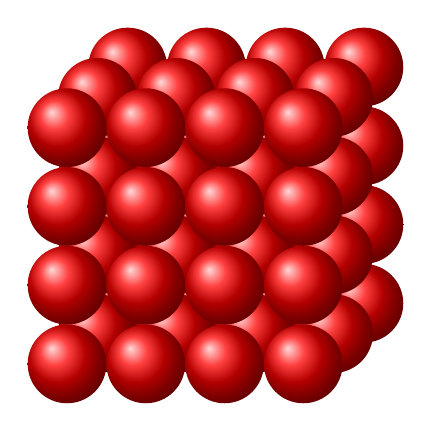
\begin{tikzpicture}
  \foreach \z in {1,2,3}{
  \foreach \i in {3,2,1,0}{% This one doesn't matter
    \foreach \j in {3,2,1,0}{% This will crate a membrane
        \shade[ball color=red] ({\i},{\j},\z) circle(0.5);
      }
    }
  }
\end{tikzpicture}
\subcaption{} \label{fig:M1}
\end{subfigure}%
\par\bigskip

\begin{subfigure}{1.0\linewidth}
\centering
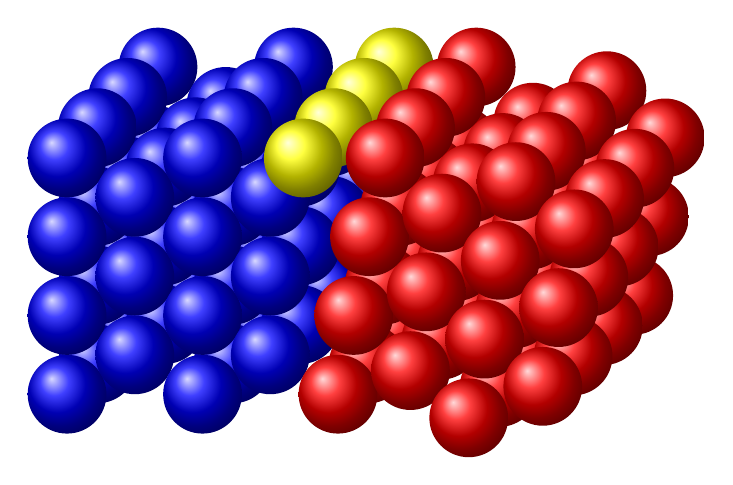
\begin{tikzpicture}
    \foreach \x in {0,1,2,3}{%
      \foreach \z in {0,1,2,3}{%
      \shade[ball color=blue] (0,\x,\z) circle(0.5);
      }
    }
    \foreach \x in {0.5,1.5,2.5}{%
      \foreach \z in {0,1,2,3}{%
      \shade[ball color=blue] ({1*sqrt(0.74)},\x,\z) circle(0.5);
      }
    }
    \foreach \x in {0,1,2,3}{%
      \foreach \z in {0,1,2,3}{%
      \shade[ball color=blue] ({2*sqrt(0.74)},\x,\z) circle(0.5);
      }
    }
    \foreach \x in {0.5,1.5,2.5}{%
      \foreach \z in {0,1,2,3}{%
      \shade[ball color=blue] ({3*sqrt(0.74)},\x,\z) circle(0.5);
      }
    }
    \foreach \z in {0,1,2,3}{%
      \shade[ball color=yellow] ({3},3,\z) circle(0.5);
    }
    \foreach \y in {0,1,2,3}{%
      \foreach \z in {0,1,2,3}{%
      \shade[ball color=red] ({4*sqrt(0.74)+0.2*\y},\y,\z) circle(0.5);
      }
    }
    \foreach \y in {0.3,1.3,2.3}{%
      \foreach \z in {0,1,2,3}{%
      \shade[ball color=red] ({5*sqrt(0.74)+0.2*\y},\y,\z) circle(0.5);
      }
    }
    \foreach \y in {-0.3,0.7,1.7,2.7}{%
      \foreach \z in {0,1,2,3}{%
      \shade[ball color=red] ({6*sqrt(0.74)+0.2*\y},\y,\z) circle(0.5);
      }
    }
    \foreach \y in {0.1,1.1,2.1}{%
      \foreach \z in {0,1,2,3}{%
      \shade[ball color=red] ({7*sqrt(0.74)+0.2*\y},\y,\z) circle(0.5);
      }
    }


\end{tikzpicture}
\subcaption{} \label{fig:M2}
\end{subfigure}%
\par\bigskip

\begin{subfigure}{1.0\linewidth}
\centering
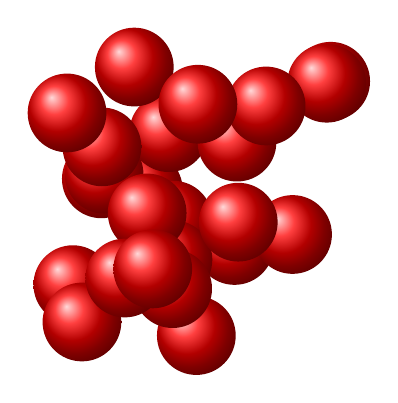
\begin{tikzpicture}
  \foreach \z in {0,...,24}{
    \shade[ball color=red] ({rand*1.5},{rand*1.5},{rand*1.5}) circle(0.5);
  }
\end{tikzpicture}
\subcaption{} \label{fig:M3}
\end{subfigure}
\par\bigskip
\caption{Different degrees of ordered structures, where (a) is a crystalline of a simple cubic lattice, (b) is a polycrystalline of a hexagonal lattice, and (c) is an amorphous. }
\label{fig:crystalstructure}
\end{figure}


\newpage
One example of a crystal structure is the perovskite structure. Compounds with this structure are characterized by having an $ABX_3$ stoichiometry whose symmetri belong to one of 15 space groups identified by Lufaso \& Woodward \cite{Lufaso2001}, such as the cubic, orthorombic and tetragonal. For our purpose, we will be looking into when the X atom is oxygen, and refer to the oxygen-perovskite $ABO_3$. The A atom is nine- to 12-fold coordinated by oxygen, while the B atom is sixfold coordinated by oxygen, and the $BO_6$ octahedra are connected to the corners in all three directions as visualized in figure \ref{fig:perovskite}.

\begin{wrapfigure}{r}{0.5\textwidth}
  \centering
  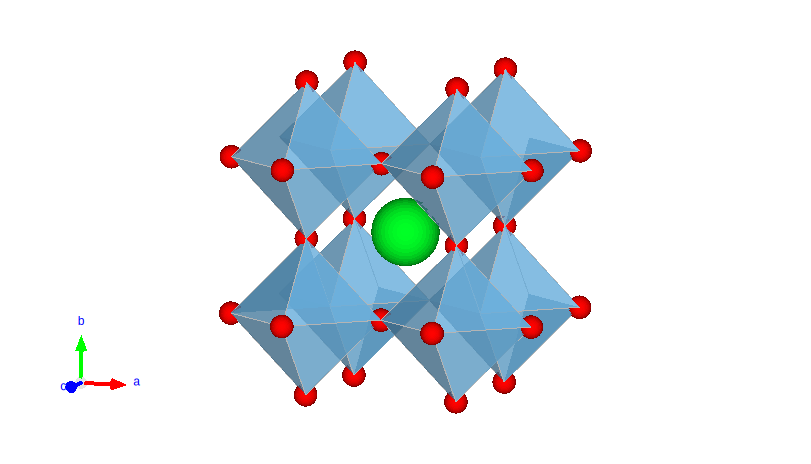
\includegraphics[width=0.48\textwidth]{theory/figures/SrTiO3_mp-5229_primitive.pdf}
  \caption{A crystal structure of SrTiO$_3$ which is a cubic perovskite. The red atoms are oxygen, whereas the green atom is strontium, and inside every corner-sharing BO$_6$ octahedral unit is a titanium atom.}
  \label{fig:perovskite}
\end{wrapfigure}

The motivation behind the research on perovskites is related to the large amount of available ABO$_3$ chemistries, where a significant portion of these take the perovskite structure. Perovskites have a broad specter of applications, ranging from high-temperature superconductors \cite{Bednorz1988} and ionic conductors \cite{Boivin1998} to multiferroic materials \cite{Cheong2007}. Additionally, adding a perovskite-type compound to solar cells has reportedly resulted in higher performance efficiencies while being cheap to produce and simple to manufacture \cite{IbnMohammed2017, Chen2014}. However, this includes the use of hybrid organic-inorganic compounds and excludes the use of oxygen.

%Point defects are the type of defect that can be utilised in generating a qubit, thus being a special interest for this thesis. They can arise as either a vacancy in the lattice, interstitial placement inbetween lattice sites, or as a substitution of an existing atom in the lattice.

Her kan jeg skrive videre om NV -1 strukturen og defekten, da den blir brukt senere.

\clearpage
\section{Introduction to semiconductor physics}

Isolated atoms have distinct energy levels, where the Pauli exlusion principle \cite{Pauli1925} states for fermions that each energy level can at most accomodate two electrons of opposite spin. In a solid, the discrete energy levels of the isolated atom spread into continuous energy bands since the wavefunctions of the electrons in the neighboring atoms overlap. Hence, an electron is not neccessarily localized at a particular atom anymore. Every material has a unique band structure, similar to every human having their unique fingerprint.


\begin{wrapfigure}{r}{0.35\textwidth}
  \begin{minipage}{\linewidth}
    \centering\captionsetup[subfigure]{justification=centering}
  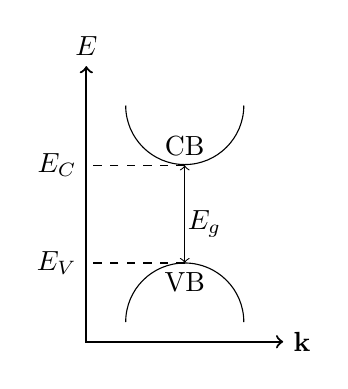
\begin{tikzpicture}[scale=1]
      \draw [<->,thick] (0,3.5) node (yaxis) [above] {$E$}
          |- (2.5,0) node (xaxis) [right] {$\textbf{k}$};
      \draw (0.5,0.25) arc(180:0:0.75cm);
      \draw (2.0,3.0) arc(0:-180:0.75cm);
      \coordinate (VB) at (1.25,1.0);
      \coordinate (CB) at (1.25,2.24);
      \draw[<->] (CB) node[above] {CB}
        -| (VB) node[below] {VB};
      \draw[dashed] (VB) -- (0,1.0) node[left]{$E_V$};
      \draw[dashed] (CB) -- (0,2.24) node[left]{$E_C$};
      \node at (1.5,1.5) {$E_g$};
  \end{tikzpicture}
  \subcaption{}
  \label{fig:directbandgap}
  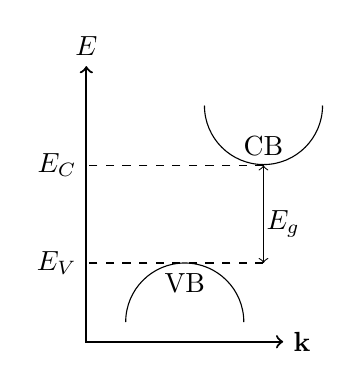
\begin{tikzpicture}[scale=1]
      \draw [<->,thick] (0,3.5) node (yaxis) [above] {$E$}
          |- (2.5,0) node (xaxis) [right] {$\textbf{k}$};
      \draw (0.5,0.25) arc(180:0:0.75cm);
      \draw (3.0,3.0) arc(0:-180:0.75cm);
      \coordinate (VB) at (2.25,1.0);
      \coordinate (CB) at (2.25,2.24);
      \draw[<->] (CB) node[above] {CB}
        -| (VB);
      \draw[dashed] (VB) -- (0,1.0) node[left]{$E_V$};
      \draw[dashed] (CB) -- (0,2.24) node[left]{$E_C$};
      \node at (2.5,1.5) {$E_g$};
      \node at (1.25,0.75) {VB};
  \end{tikzpicture}
  \label{fig:indirectbandgap}
  \subcaption{}
  \end{minipage}
  \caption{A schematic drawing of a (a) direct bandgap and an (b) indirect bandgap.}
\end{wrapfigure}


Knowing which energy bands are occupied by electrons is the key in understanding the electrical properties of solids. The highest occupied electron band at $0$ K is called the valence band (VB), while the lowest unoccupied electron band is called the conduction band (CB). The energy gap of forbidden energy levels between the maximum VB and the minimum CB is known as the band gap, and its energy is denoted as $E_g$. If a material can be classified as a semiconductor depends on the band gap and the electrical conductivity. As an example, Silicon is commonly thought of as a semiconductor, and has a band gap of about $1.12$ eV at $275$ K \cite{Martienssen2005}.

To be able to accelerate electrons in a solid using an electrical field, they must be able to move into new energy states. At $0$ K, the entire valence band of a semiconductor is full with electrons and there are no available states nearby, making it impossible for current to flow through the material. This can be solved by using either thermal or optical energy to excite electrons from the valence band to the conduction band, in order to \textit{conduct} electricity. At room temperature, some semiconductors will have electrons excited to the conduction band solely from thermal energy matching the energy band gap \cite{BenStreetman2015}.

In some scenarios, thermal or optical energy is not sufficient for an excitation since the energy bands are also dependent on the crystal momentum. A difference in the momentum of the minimal-energy state in the conduction band and the maximum-energy state in the valence band results in an \textit{indirect bandgap} as seen in figure \ref{fig:indirectbandgap}. If there is no difference at all, the material has a \textit{direct bandgap}, which is visualized in figure \ref{fig:directbandgap}.

Electrons in semiconductor materials can be described according to the Fermi-Dirac distribution
\begin{align*}
  f(E) = \frac{1}{1+e^{(E-E_F)/kT}},
\end{align*}
where $k$ is Boltzmann's constant, $T$ is temperature, $E$ is the energy and $E_F$ is the Fermi level. The Fermi-Dirac distribution gives the probability that a state will be occupied by an electron, and at $T=0$ K, every energy state lower than $E_F$ is occupied by electrons while the opposite is true for energy states above $E_F$ \cite{BenStreetman2015}.

\section{Point defects in semiconductors}

In real life, a perfect crystal without any symmetry-breaking flaw does not exist. These flaws are known as defects and can occur up to three dimensions. An example one-dimensional defect is known as a \textit{line defect}, while two dimensional defects can be \textit{planar defects}, and in three dimensions we have \textit{volume defects}. Lastly, defects can also occur in zero dimensions and are then termed \textit{point defects}. Point defects normally occur as either vacancies, interstitial placement inbetween lattice sites or as substitution of another existing atom in the lattice.

Defects can greatly influence both the electronic and optical propertires of a material. A substitional defect can at first be regarded as an impurity or an antisite, but they can also be intentionally inserted, an approach known as \textit{doping}. Doping can result in an excess of electrons or holes, making the semiconductor either an n- or p-type, respectively. Consequently, the semiconductor will have energy levels in the (forbidden) band gap that originates from the defects. If the energy levels introduced are closer than $ \sim 0.2$ eV to the band egdes, they are termed \textit{shallow} defects.

Shallow defects can contribute with either excess electrons to the conduction band, or excess holes to the valence band. However, the induced charge carriers (electrons or holes) interact strongly with the band egdes, resulting in a delocalized wavefunction regarding the position in the lattice. %For the latter scenario, shallow defects are commonly labelled as \textit{dopants}.

For the opposite case, if the energy levels rests closer to the middle of the semiconductor's gap, the introduced defects are known as \textit{deep level} defects. Deep levels normally occur due to either dangling bonds or impurities, and have highly localized electron wavefunctions. This might assure the isolation required for long coherence times, which is an appealing promise in quantum technological advances.

Deep levels are in general unfortunate in semiconductors since they can interact with the charge carriers, potentially destroying the desired electronic or optical property of the material. Deep level defects can function as  electron-hole recombination centers, or to trap charge carriers, yielding the commonly used name deep level \textit{traps}. Both situations results in a lower concentration of charge carriers, which showcase why deep levels can be unwanted in semiconductor devices.






\section{Qubit host candidates}

%We have showed several criteria for identifying

Weber \textit{et al.} \cite{Weber2010} proposed in 2010 four criteria that should be met for a solid-state semiconductor material hosting a qubit defect. An ideal crystalline host should have \cite{Weber2010}
\begin{itemize}
  \item[(H1)] A wide band gap to accomodate a deep center.
  \item[(H2)] Small spin-orbit coupling in order to avoid unwanted spin flips in the defect bound states.
  \item[(H3)] Availability as high-quality, bulk, or thin-film single crystals.
  \item[(H4)] Constituent elements with naturally occuring isotopes of zero nuclear spin.
\end{itemize}

Host candidates that satisfy criteria (H1) and (H2) can be found by studying the electronic structure of the compounds. What tends to happen for defects in semiconductors, is that the electronic states associated with the defect have energies that lie within the (forbidden) band gap of the semiconductor. This is schematically drawn and explained for diamond in figure (\ref{fig: diamond electronic structure}). A large band gap can accomodate multiple highly isolated states and make them confined and isolated from interactions with the environment, which is favorable for longer coherence times. However, the desired band gap depends on the application, since the Fermi level of large band gap materials is challenging to control \cite{Bassett2019}.

Table (\ref{tab:qubithosts}) lists several material host candidates that exhibit promising band gap capable of accommodating a deep level defect. The spin-orbit splitting is an indication of the strength of the spin-orbit interaction, and is taken at the $\Gamma$ point from the valence-band splitting. A smaller value may indicate less susceptibility to decoherence.

Criterion (H3) is important for scalability and further potential for a large-scale fabrication. The given candidate hosts provided in table (\ref{tab:qubithosts}) can all be grown as single crystals, but with varying quality and size.

Normally, nuclear spin is a major source of decoherence for all semiconductor-based quantum technologies. This would exclude the use of all elements in odd groups in the periodic table, since these elements exhibit nonzero nuclear spin. As a result, the spin-coherence time of a paramagnetic deep center \cite{Weber2010} might increase. However, nuclear spin can also induce additional quantum degrees of freedom for applications in the right configuration \cite{Bassett2019}. Therefore, criterion (H4) is not a strict requirement but is a general recommendation for reducing decoherence time.  %Therefore, we will not completely exclude all nonzero nuclear spin elements from our list.

Weber \textit{et al} \cite{Weber2010} use criteria $(H1)-(H4)$ to specifically find analogies to the $NV^{-1}$ center in other material systems, thus leaving the discussion of other criteria out, such as the choice of crystal system. The atomic configuration and crystal structure of a material strongly influences the properties of a defect, since a defect's orbital and spin structure is dependent on its spatial symmetry \cite{Bassett2019}. In particular, it is the point group that decides which multiplicity a given energy level should have \cite{James1976}. A higher defect symmetry group generally facilitates degenerate states, which may give rise to high spin states according to Hund's rules. This is a favorable trend, since high spin states allows for coherent spin control in addition to the chance of generating spin-photon entanglement \cite{Bassett2019, Togan2010}. Inversion symmetry in the host crystal can also be beneficial, resulting in reduced inhomogenous broadening and spectral diffusion of optical transitions as a consequence of being generally insensitive to external electric fields \cite{Bassett2019}.

\begin{figure}[ht!]
  \centering
\begin{subfigure}{1.0\linewidth}
\centering
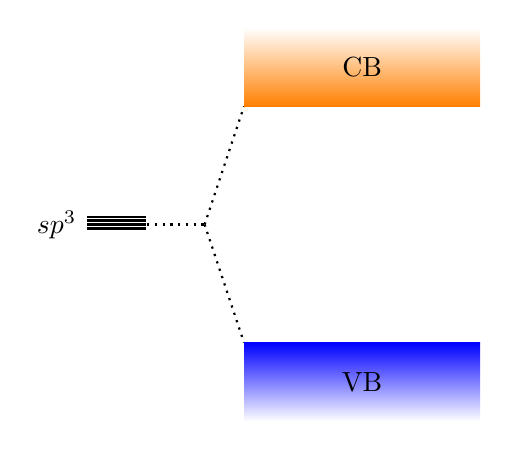
\begin{tikzpicture}

  \atom[name=C, color=orange, pos={(-2,0)},scale=0.5]{
    gray/45/45/0,
    gray/315/315/0,
    gray/225/225/0,
    gray/135/135/0}

  \draw[thick,-] (-1.25,-4) -- (-2.0,-4) node[anchor=east]{$sp^3$};
  \draw[thick,-] (-1.25,-3.95) -- (-2.0,-3.95);
  \draw[thick,-] (-1.25,-4.05) -- (-2.0,-4.05);
  \draw[thick,-] (-1.25,-3.90) -- (-2.0,-3.90);

  \draw[thick, dotted] (-1.23,-4) -- (-0.5,-4);
  \draw[thick, dotted] (-0.5,-4) -- (0,-5.5);
  \draw[thick, dotted] (-0.5,-4) -- (0,-2.5);

  %\node at (1.5,1.5) {$E_g$};
  %\draw (0,-1.5) -- (2,-1.5) -- (2,-2) -- (0,-2) -- (0,0);
  \shade[top color=white,bottom color=orange] (0,-2.5) rectangle (3.0,-1.5) node[pos=.5] {CB};
  \shade[top color=blue,bottom color=white] (0.,-6.5) rectangle (3.0,-5.5) node[pos=.5] {VB};

  \atom[name=C, color=orange, scale=0.5]{
    gray/45/45/0,
    gray/315/315/0,
    gray/225/225/0,
    gray/135/135/0}
  \atom[name=C, color=orange, pos={(0.75,0.75)},scale=0.5]{
    gray/45/45/0,
    gray/315/315/0,
    gray/225/225/0,
    gray/135/135/0}
  \atom[name=C, color=orange, pos={(1.5,0)},scale=0.5]{
    gray/45/45/0,
    gray/315/315/0,
    gray/225/225/0,
    gray/135/135/0}
  \atom[name=C, color=orange, pos={(0.75,-0.75)},scale=0.5]{
    gray/45/45/0,
    gray/315/315/0,
    gray/225/225/0,
    gray/135/135/0}
  \atom[name=C, color=orange, pos={(2.25,0.75)},scale=0.5]{
    gray/45/45/0,
    gray/315/315/0,
    gray/225/225/0,
    gray/135/135/0}
  \atom[name=C, color=orange, pos={(2.25,-0.75)},scale=0.5]{
    gray/45/45/0,
    gray/315/315/0,
    gray/225/225/0,
    gray/135/135/0}
  \atom[name=C, color=orange, pos={(3.0,0)},scale=0.5]{
      gray/45/45/0,
      gray/315/315/0,
      gray/225/225/0,
      gray/135/135/0}

\end{tikzpicture}
\subcaption{} \label{fig:diamond structure}
\end{subfigure}%

\begin{subfigure}{1.0\linewidth}
\centering
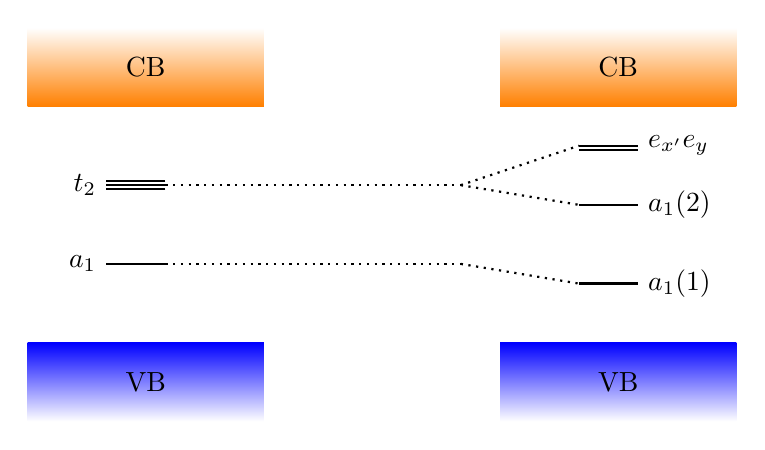
\begin{tikzpicture}

  \shade[top color=white,bottom color=orange] (0.-7,-2.5) rectangle (3.0-7,-1.5) node[pos=.5] {CB};
  \shade[top color=blue,bottom color=white] (0.-7,-6.5) rectangle (3.0-7,-5.5) node[pos=.5] {VB};

  \draw[thick,-] (1.75-7,-4.5) -- (1.0-7,-4.5) node[anchor=east]{$a_1$};
  \draw[thick,-] (1.75-7,-3.5) -- (1.0-7,-3.5) node[anchor=east]{$t_2$};
  \draw[thick,-] (1.75-7,-3.55) -- (1.0-7,-3.55);
  \draw[thick,-] (1.75-7,-3.45) -- (1.0-7,-3.45);

  \atom[name=C, color=orange, pos={(0-7,0)}, scale=0.5]{
    gray/45/45/0,
    gray/315/315/0,
    gray/225/225/0,
    gray/135/135/0}
  \atom[name=C, color=orange, pos={(0.75-7,0.75)},scale=0.5]{
    gray/45/45/0,
    red/315/315/0,
    gray/225/225/0,
    gray/135/135/0}
  \atom[name=v, color=gray, pos={(1.5-7,0)},scale=0.5]{}
  \atom[name=C, color=orange, pos={(0.75-7,-0.75)},scale=0.5]{
    red/45/45/0,
    gray/315/315/0,
    gray/225/225/0,
    gray/135/135/0}
  \atom[name=C, color=orange, pos={(2.25-7,0.75)},scale=0.5]{
    gray/45/45/0,
    gray/315/315/0,
    red/225/225/0,
    gray/135/135/0}
  \atom[name=C, color=orange, pos={(2.25-7,-0.75)},scale=0.5]{
    gray/45/45/0,
    gray/315/315/0,
    gray/225/225/0,
    red/135/135/0}
  \atom[name=C, color=orange, pos={(3.0-7,0)},scale=0.5]{
      gray/45/45/0,
      gray/315/315/0,
      gray/225/225/0,
      gray/135/135/0}

    \shade[top color=white,bottom color=orange] (0.-1.,-2.5) rectangle (3.0-1.0,-1.5) node[pos=.5] {CB};
    \shade[top color=blue,bottom color=white] (0.-1.,-6.5) rectangle (3.0-1.0,-5.5) node[pos=.5] {VB};

    \atom[name=C, color=orange, pos={(0.-1.,0)}, scale=0.5]{
      gray/45/45/0,
      blue/315/315/0,
      gray/225/225/0,
      gray/135/135/0}
    \atom[name=C, color=orange, pos={(0.75-1,0.75)},scale=0.5]{
      gray/45/45/0,
      red/315/315/0,
      gray/225/225/0,
      gray/135/135/0}
    \atom[name=v, color=gray, pos={(1.5-1,0)},scale=0.5]{}
    \atom[name=N, color=green!95, pos={(0.75-1,-0.75)},scale=0.5]{
      blue/45/45/0,
      blue/315/315/0,
      blue/225/225/0,
      blue/135/135/0}
    \atom[name=C, color=orange, pos={(2.25-1,0.75)},scale=0.5]{
      gray/45/45/0,
      gray/315/315/0,
      red/225/225/0,
      gray/135/135/0}
    \atom[name=C, color=orange, pos={(2.25-1,-0.75)},scale=0.5]{
      gray/45/45/0,
      gray/315/315/0,
      gray/225/225/0,
      red/135/135/0}
    \atom[name=C, color=orange, pos={(3.0-1,0)},scale=0.5]{
        gray/45/45/0,
        gray/315/315/0,
        gray/225/225/0,
        gray/135/135/0}

    \draw[thick, dotted] (1.75-7,-3.5) -- (-1.5,-3.5);
    \draw[thick, dotted] (-1.5,-3.5) -- (0,-3.0);
    \draw[thick, dotted] (-1.5,-3.5) -- (0,-3.75);

    \draw[thick,-] (1.0-1,-3.0) -- (1.75-1,-3.0) node[anchor=west]{$e_{x'}e_y$};
        \draw[thick,-] (1.75-1,-3.05) -- (1.0-1,-3.05);
    \draw[thick,-] (1.0-1,-3.75) -- (1.75-1,-3.75) node[anchor=west]{$a_1(2)$};

    \draw[thick, dotted] (1.75-7,-4.5) -- (-1.5,-4.5);
    \draw[thick, dotted] (-1.5,-4.5) -- (0,-4.75);
    \draw[thick,-] (1.0-1,-4.75) -- (1.75-1,-4.75) node[anchor=west]{$a_1(1)$};

\end{tikzpicture}
\subcaption{} \label{fig:defect diamond structure}
\end{subfigure}
\par\bigskip
\caption{A schematic representation of the electronic structure of a point defect in a tetrahedrally coordinated semiconductor, exemplified by diamond. Panel (a) shows the electronic states that correspond to the difference for an isolated atom and a lattice of atoms, as a superposition of $sp^3$ orbitals that generates valence and conduction bands. In panel (b), a vacancy has been created by removing a carbon atom, and the four orbitals interact with each other resulting in two new states with $a_1$ and $t_2$ symmetry. The carbon atoms interact stronger with each other than the remaining four orbitals, which is why the two new states rests within the semiconductor's band gap. Figure used from Ref. \cite{Gordon2013}.}
\label{fig: diamond electronic structure}
\end{figure}


%In fact, all of the criteria could be regarded as recommendations,

\begin{table}[!ht]
\centering
\noindent\makebox[\textwidth]{
\begin{tabular}{M{2.5cm} M{2.5cm} M{3.0cm} M{4.0cm}}
  \hline
  \hline
  Material & Band gap  $E_g$ (eV) & Spin-orbit splitting $\Delta_{so}$ (meV) & Stable spinless nuclear isotopes? \\
  \hline
  3C-SiC & 2.39 & 10 & Yes \\
  4C-SiC & 3.26 \cite{Neudeck1995} & 6.8 & Yes \\
  6C-SiC & 3.02 & 7.1 & Yes \\
  AlN & 6.13 & 19 \cite{Silveira2005} & No \\
  GaN & 3.44 & 17.0 & No \\
  AlP & 2.45 & 50 \cite{Lawaetz1971} & No \\
  GaP & 2.27 & 80 & No \\
  AlAs & 2.15 & 275 & No \\
  ZnO & 3.44 \cite{Beckers1998} & -3.5 & Yes \\
  ZnS & 3.72 \cite{Kumbhojkar2000} & 64 & Yes \\
  ZnSe & 2.82 & 420 & Yes \\
  ZnTe & 2.25 & 970 & Yes \\
  CdS & 2.48 & 67 & Yes \\
  \hline
  C (Diamond) & 5.5 & 6 & Yes \\
  Si & 1.12 & 44 & Yes \\
  \hline
  \hline
\end{tabular}
}
\caption{Table taken from Gordon \textit{et al.} \cite{Gordon2013} that lists a number of tetrahedrally coordinated hosts whose band gaps are larger than $2.0$ (eV), and compares it to diamond and Si. All experimental values are from Ref. \cite{Martienssen2005}, except for where explicity cited otherwise. For materials where more than one structure is stable in room temperature, the most dominant room-temperature phase's band parameters are chosen.}
\label{tab:qubithosts}
\end{table}

%When isolated atoms are brought together to form a solid, various interactions occur between neighboring atoms. These interactions are the basis that forms the varied electrical properties of solids. . Each energy level

%The interactions between the electrons in a solid defines what kind of bonding there is, and can result in ionic bonding, metallic bonding or covalent bonding alone or mixed together.


 %A solid that conducts electrical current is, by definition, a metal. Every solid that has its own characteristic energy

 %On the other hand, a material that does not conduct electrical current is an insulator.

 \newpage

        %\chapter{Introduction to quantum mechanics}

To fully understanding the underlying physics behind computational material science, we will need to investigate how we can calculate the forces acting inside a crystal. Since these forces are happening on a microscopic scale, we will need to utilise the theory of quantum mechanics.

In this thesis, we will ony summarize the neccessary theory behind density functional theory, leaving most of the quantum-mechanical world untouched. However, the fundamental theory remains the same and we will start our venture with the Schrödinger equation.

%canonical variables
%dynamical variables
%operator
%canonical substitusion

\begin{comment}
\section{The single-electron Schrödringer equation}

We will start of investigating the Schrödinger equation with only one electron \cite{Griffiths2017}
\begin{align}
    i\hslash \frac{\partial \Psi}{\partial t} = -\frac{\hslash^2}{2m}\nabla^2 \Psi + V\Psi
    \label{eq:Schrödinger}
\end{align}
for a convenient external potential $V_{ext}(r)$ that is independent of time. We will try to look for solutions for (\ref{eq:Schrödinger}) by separating the wave function into a space-dependent and time-dependent function
%Most wavefunctions are solutions to (\ref{eq:Schrödinger}), but if the wavefunction describes a stationary state, the wavefunction has to be an eigenfunction to H for reasons that will become clear shortly.
\begin{align}
  \Psi(r,t) = \psi(r)\phi(t).
  \label{eq:separation}
\end{align}
By inserting ordinary derivatives and dividing each side with equation (\ref{eq:separation}), our Schrödinger equation (\ref{eq:Schrödinger}) now reads
\begin{align}
  i\hslash \frac{1}{\phi(t)}\frac{d\phi(t)}{dt} = - \frac{\hslash^2}{2m} \frac{1}{\psi(r)}\nabla^2 \psi + V(r)
\end{align}

Since the potential function $V(r)$ is independent of time, we observe the time and space dependencies of each side and state the fact that both sides has to be constant. Thus, two intriguing equations unveil themselves;
%captivating?
\begin{align}
  i\hslash \frac{1}{\phi(t)}\frac{d\phi(t)}{dt} = E\phi(t)
  \label{eq:time}
\end{align}
and
\begin{align}
  \frac{\hslash^2}{2m} \frac{1}{\psi(r)}\nabla^2 \psi + V(r) = E\psi(r)
  \label{eq:tise}
\end{align}
where the first equation (\ref{eq:time}) has a general solution $\phi(t) = C \exp (-iEt/\hslash)$ and $C=1$ after normalization, and the second equation (\ref{eq:tise}) is known as time-independent Schrödinger equation. These two equations are connected through the variable $\varepsilon$.

By utilizing variable separation to get equation (\ref{eq:separation}), we find that the wavefunction is describing a stationary state with probability density
\begin{align*}
  \lvert \Psi (r,t)\rvert ^2 &= \Psi^*\Psi \\
  &= \Psi^* e^{iEt/\hslash} \Psi e^{-i Et/\hslash} \\
  &= \lvert \Psi (r)\rvert ^2
\end{align*}
that is independent of time. Conveniently, this is also true for every expectation value; they are all constant in time. We can also try to express this in classical terms regarding the Hamiltonian, which in this scenario is defined as
\begin{align}
    \hat{H}(r, p) = \frac{p^2}{2m} + V(r) = -\frac{\hslash^2}{2m}\nabla^2 + V(r)
\end{align}
simplifying equation \ref{eq:tise} to
\begin{align}
  \hat{H} \psi = E\psi
  \label{eq:tise_nesten}
\end{align}
and we can find the expectation value of the total energy as
\begin{align*}
    \langle H \rangle &= \int \psi^* \hat{H} \psi dr \\
                &= E\int \lvert \Psi \rvert ^2 dr \\
                &= E
\end{align*}
using the fact that expectation values are constant in time for stationary states. Similarly, we can try to estimate the variance of the Hamiltonian,
\begin{align*}
  \sigma_H^2 &= \langle H^2 \rangle - \langle H \rangle ^2 \\
            &= E^2 - E^2 \\
            &= 0
\end{align*}
which appropiately describes that every measurement of the total energy is certain to return the value E.

\subsection{Eigenfunctions}
So far, we have not given an explanation of what a wavefunction is. As a matter of fact, we have actually found an eigenfunction
\begin{align*}
  \psi_\kappa(r,t) = \psi_\kappa e^{-i\varepsilon_\kappa t/\hslash}
\end{align*}
where $\kappa$ denotes the $k$-th eigenfunction and $\varepsilon_\kappa$ is its corresponding energy eigenvalue. The eigenfunctions have distinct energies and have the attribute that they are orthogonal and normalized with respect to
\begin{align*}
  \bra{\psi_\kappa (r,t)} \ket{\psi_{\kappa`} (r,t)} = \delta_{\kappa \kappa'}.
\end{align*}
The state with the lowest energy is called the ground state, and is where it is most likely to find an electron in a single-electron system with no external potential applied.

A general wavefunction can be generated by a summation of eigenfunctions (such as the eigenfunction in the latter case)
\begin{align}
\Psi(r,t) = \sum_\kappa c_\kappa \psi_{\kappa}(r,t),
\end{align}
where $c_\kappa$ is a constant. A general wavefunction does not neccessarily describe stationary states, and consequently does not have distinct energies but is rather represented statistically from the expectation value
\begin{align*}
  E = \sum_{\kappa} \lvert c_\kappa \rvert \varepsilon_\kappa.
\end{align*}
Solving Schrödinger equation for a general wavefunction is rather troublesome. Fortunately, we can use the eigenfunctions instead, transforming equation \ref{eq:tise_nesten} into time-independent Schrödinger equation for eigenfunctions
\begin{align}
  \hat{H} \psi_{\kappa}(r) = \varepsilon_\kappa \psi_\kappa(r).
\end{align}

The shape of en eigenfunction has normally high spatial symmetri that depends on the symmetri of the potential $V_{ext}(r)$ and the boundary conditions \cite{Persson2020}. The study of how atoms in a crystalline interact with each other is of upmost importance when trying to explain macroscopic consequences.

\end{comment}

\section{The Schrödinger equation}

In principle, we can describe all physical phenomenas of a system with the wavefunction $\Psi(\textbf{r},t)$ and the Hamiltonian $\hat{H}(\textbf{r},t)$, where $\textbf{r}$ is the spatial position and $t$ is the time. Unfortunately, analytical solutions for the the time-dependent Schrödinger equation,
\begin{align}
    i\hslash \frac{\partial}{\partial t} \Psi(\textbf{r},t) = \hat{H}(\textbf{r},t) \Psi(\textbf{r},t),
    \label{eq:tdse}
\end{align}
are extremely rare. More conveniently, we can generate a general wavefunction by a summation of eigenfunctions,
\begin{align}
  \Psi(\textbf{r},t) = \sum_\kappa c_\kappa \psi_\kappa(\textbf{r},t),
\end{align}
where $c_\kappa$ is a constant and $\psi_\kappa$ is the $\kappa$-th eigenfunction. A general wavefunction does not neccessarily describe stationary states, and consequently does not have distrinct energies but is rather represented statistically from the expectation value
\begin{align}
  E = \sum_\kappa \lvert c_\kappa \rvert E_\kappa.
\end{align}

 Solving the Schrödinger equation for a general wavefunction is rather troublesome, but luckily we can use the eigenfunctions instead, transforming equation \ref{eq:tdse} into the time-independent Schrödinger equation for eigenfunctions
\begin{align}
  \hat{H}\psi_\kappa(\textbf{r}) = E_\kappa \psi_k(\textbf{r}),
\end{align}
where $E_\kappa$ is the eigenvalue of the $\kappa$-th eigenstate $\psi_\kappa(\textbf{r})$. The eigenfunctions have distinct energies, and the state with the lowest energy is called the ground state. They have the attribute that they are orthogonal and normalized with respect to
\begin{align}
  \left \langle \psi_\kappa \left(\textbf{r}\right) \rvert \psi_{\kappa`} \left(\textbf{r} \right) \right \rangle = \delta_{\kappa \kappa'}.
\end{align}
The symmetry of an eigenfunction depends on the symmetry of the potential $V_{ext}(\textbf{r})$ and the boundary conditions \cite{Persson2020}.

\section{The many-particle Schrödinger equation}
As we extend the theory to include many-particle systems, we will gradually explain and add the different contributions that make up the many-body Hamiltonian. During this process, we will neglect any external potential applied to the system.

If we place a simple electron with mass $m_e$ in its own system, it will be in  possession of kinetic energy. Instead of just one electron, we can place $N_e$ electrons, and they will together have the total kinetic energy
\begin{align}
  T_e = - \sum_{j=1}^{N_e} \frac{\hslash^2\nabla_j}{2m_e}.
\end{align}
All the electrons are negatively charged, causing repulsive Coulomb interactions between each and every electron, totalling to
\begin{align}
  U_{ee} = \sum_{j=1}^{N_e}\sum_{j'<j} \frac{q^2}{\lvert r_j - r_{j'}\rvert}.
  \label{eq:electron-electron}
\end{align}
The summation voids counting each interaction more than once. Simultaneously, we can place $N_n$ nuclei with mass $m_n$ in the same system, accumulating the kinetic energy
\begin{align}
  T_n = - \sum_{a=1}^{N_n} \frac{\hslash^2\nabla_a}{2m_n}.
\end{align}
As in the example with electrons, the nuclei are also experiencing repulsive interactions between every single nucleus, adding up the total interactions as
\begin{align}
  U_{nn} = \sum_{a=1}^{N_n}\sum_{a'<a} \frac{q^2 Z_aZ_{a'}}{\lvert R_a - R_{a'}\rvert }.
\end{align}
where $Z_a$ is the atom number of nuclei number $a$.

The system now contains $N_e$ electrons and $N_n$ nuclei, thus we need to include the attractive interactions between the them,
\begin{align}
  U_{en} = - \sum_{j=1}^{N_e} \sum_{a=1}^{N_n} \frac{q^2Z_a}{\lvert r_j-R_a\rvert}.
\end{align}

Together, these equations comprise the time-independent many-particle Hamiltonian
\begin{align}
  \begin{aligned}
    \hat{H} = &- \sum_{j=1}^{N_e} \frac{\hslash^2\nabla_j}{2m_e} - \sum_{a=1}^{N_n} \frac{\hslash^2\nabla_a}{2m_n} + \sum_{j=1}^{N_e}\sum_{j'<j} \frac{q^2}{\lvert r_j - r_{j'}\rvert} \\ &+\sum_{a=1}^{N_n}\sum_{a'<a} \frac{q^2 Z_aZ_{a'}}{\lvert R_a - R_{a'}\rvert } - \sum_{j=1}^{N_e} \sum_{a=1}^{N_n} \frac{q^2Z_a}{\lvert r_j-R_a\rvert}.
  \end{aligned}
\end{align}


A few problems arise when trying to solve the many-particle Schrödinger equation. Firstly, the amount of atoms in a crystal is very, very massive. As an example, we can numerically try to calculate the equation \ref{eq:electron-electron} for a $1$mm$^3$ silicon-crystal that contains $7\cdot 10^{20}$ electrons. For this particular problem, we will pretend to use the current fastest supercomputer Fugaku \cite{Top500} that can calculate $514$ TFlops, and we will assume that we need $2000$ Flops to calculate each term inside the sum \cite{Persson2020}, and we need to calculate it $N_e \cdot N_e/2$ times for the (tiny) crystal. The entire electron-electron interaction calculation would take $2.46 \cdot 10^{19}$ years to finish for a tiny crystal. Thus, the large amount of particles translates into a challenging numerical problem.

%In one cubic-centimeter of a crystal, there are around $10^{23}$ electrons. This number is roughly the same as the number of stars in the universe, grain of sand on all beaches in the world, or currently $1.41\cdot 10^{19}$ times the amount of Home and Away episodes made since 1988.

Secondly, the many-particle Hamiltonian contains operators that has to be applied to single-particle wavefunctions, and we have no prior knowledge of how $\Psi$ depends on the single-particle wavefunctions $\psi_\kappa$.


\section{The Born-Oppenheimer approximation}

The many-particle eigenfunction describes the wavefunction of all the electrons and nuclei and we denote it as $\Psi_{\kappa}^{en}$ for electrons (e) and nuclei (n), respectively. The Born-oppenheimer approximation assumes that nuclei, of substantially larger mass than electrons, can be treated as fixed point charges. According to this assumption, we can separate the eigenfunction into an electronic part and a nuclear part,
\begin{align}
  \Psi_\kappa^{en}(\textbf{r}, \textbf{R}) \approx \Psi_{\kappa}(\textbf{r}, \textbf{R})\Theta_{\kappa}(\textbf{R}),
\end{align}
where the electronic part is dependent on the nuclei. This is in accordance with the assumption above, since electrons can respond instantaneously to a new position of the much slower nucleus, but this is not true for the opposite scenario. To our advantage, we already have knowledge of the terms in the many-particle Hamiltionian, and we can begin by separating the Hamiltionian into electronic and nuclear parts:


\begin{align}
  \hat{H}^{en} = \overbrace{T_e + U_{ee} + U_{en}}^{\hat{H}^{e}} + \overbrace{T_n + U_{nn}}^{\hat{H}^{n}}.
\end{align}
Starting from the Schrödinger equation, we can formulate separate expressions for the electronic and the nuclear Schrödinger equations.

\begin{align}
  \hat{H^{en}} \Psi_\kappa^{en}(\textbf{r},\textbf{R}) &= E_\kappa^{en}\Psi_\kappa^{en}(\textbf{r},\textbf{R}) \quad \lvert \times \int \Psi^*(\textbf{r},\textbf{R}) d\textbf{r} \\
  \int \Psi_\kappa^*(\textbf{r},\textbf{R}) (\hat{H}^e + \hat{H}^n)\Psi_\kappa(\textbf{r},\textbf{R})\Theta_\kappa(\textbf{R})d\textbf{r} &= E_\kappa^{en} \underbrace{\int \Psi_\kappa ^* (\textbf{r},\textbf{R}) \Psi_\kappa (\textbf{r},\textbf{R}) d\textbf{r}}_{1} \Theta_\kappa(\textbf{R}).
\end{align}

Since $\Theta_\kappa(\textbf{R})$ is independent of the the spatial coordinates to electrons, we get $E_{\kappa}$ as the total energy of the electrons in the state $\kappa$.

\begin{align}
     E_\kappa(\textbf{R}) \Theta_k(\textbf{R}) + \int \Psi_k^*(\textbf{r},\textbf{R})H^n\Psi_k(\textbf{r},\textbf{R})\Theta_k(\textbf{R})d\textbf{r} = E_k^{en} \Theta_k(\textbf{R}).
\end{align}

Now, the final integration term can be simplified by using the product rule, which results in
\begin{align}
    \Big( T_n+T_n^{'} + T_n^{''} +U_{nn} + E_\kappa(\textbf{R}) \Big)\Theta_\kappa(\textbf{R}) = E_\kappa^{en}\Theta_\kappa (\textbf{R}).
\end{align}
If we neglect $T_n'$ and $T_n^{''}$ to lower the computational efforts, we obtain the Born-Oppenheimer approximation with the electronic eigenfunction as
\begin{align}
    \left( T_e + U_{ee} + U_{en} \right) \Psi_\kappa (\textbf{r},\textbf{R}) = E_{\kappa}(\textbf{R})\Psi_\kappa(\textbf{r},\textbf{R})
\end{align}
and the nuclear eigenfunction as
\begin{align}
    \left(T_n + U_{nn} + E_\kappa (\textbf{R}) \right) \Theta_\kappa(\textbf{R})= E_{\kappa}^{en}(\textbf{R})\Theta_\kappa(\textbf{r},\textbf{R}).
\end{align}

%These two equations are coupled together through the total energy, which is a potential in the nuclear equation.
How are they coupled, you might ask? The total energy in the electronic equation is a potential in the nuclear equation.


\section{The Hartree and Hartree-Fock approximation}
\begin{comment}
As we venture along from a one-electron system to a two-electron systen, we encounter a new wavefunction and Hamiltonian that needs to describe two particles, making the two-electron Schrödinger equation read

\begin{align}
  \Big( -\frac{\hslash^2 \nabla_1^2}{2m_e} - \frac{\hslash^2\nabla_2^2}{2m_e}+ \frac{q^2}{\lvert r_1-r_2  \rvert} + V_{ext}(r) \Big) \Psi_\kappa (r_1, r_2) = E_{\kappa} \Psi_\kappa (r_1, r_2),
\end{align}
where the two first terms are the kinetic energies of the electrons, while the third term is a potential that describes the repulsive Coloumb interaction between the two electrons. The last term is the external potential, well known from the earlier scenario with only one electron.
\end{comment}
The next question in line is to find a wavefunction $\Psi(\textbf{r},\textbf{R})$ that depends on all of the electrons in the system. The Hartre \cite{Persson2020} approximation to this is to assume that electrons can be described independently, suggesting the \textit{ansatz} for a two-electron wavefunction
\begin{align}
  \Psi_\kappa(\textbf{r}_1,\textbf{r}_2) = A \cdot \psi_1(\textbf{r}_1) \psi_2(\textbf{r}_2),
\end{align}
where $A$ is a normalization constant. This approximation simplifies the many-particle Shrödinger equation a lot, but comes with the downside that the particles are distinguishable and do not obey the Pauli exclusion principle for fermions.

The Hartree-fock approach, however, overcame this challenge and presented an anti-symmetric wavefunction that made the electrons indistinguishable \cite{Griffiths2017}:
\begin{align}
  \Psi_\kappa(\textbf{r}_1,\textbf{r}_2) = \frac{1}{\sqrt{2}}\Big( \psi_1(\textbf{r}_1) \psi_2(\textbf{r}_2)  - {\psi_1(\textbf{r}_2)\psi_2(\textbf{r}_1)}\Big).
\end{align}
For systems containing more than one particles, the factor $1/\sqrt{2}$ becomes the Slater determinant and is used to normalize the wave function.

\section{The variational principle}
So far, we have tried to make the time-independent Schrödinger equation easier with the use of an \textit{ansatz}, but we do not neccessarily have an adequate guess for the eigenfunctions and the ansatz can only give a rough estimate in most scenarios. Another approach, namely the \textit{variational principle}, states that the energy of any trial wavefunction is always an upper bound to the exact ground state energy by definition $E_0$.
\begin{align}
  E_0 = \bra{\psi_0 } H \ket{\psi_0} \leq \bra{\psi}H\ket{\psi} = E
  \label{eq:variational}
\end{align}
The eigenfunctions of $H$ form a complete set, which means any normalized $\Psi$ can be expressed in terms of the eigenstates
\begin{align}
  \Psi = \sum_n c_n \psi_n, \quad \textnormal{where} \quad H\psi_n = E_n \psi_n
\end{align}
for all $n = 1,2, ...$. The expectation value for the energy can be calculated as
\begin{align*}
  \bra{\Psi}H\ket{\Psi} &= \bra{\sum_{n}c_n \psi_n} H \ket{\sum_{n'} c_{n'}\psi_{n'}} \\
  &= \sum_n \sum_{n'} c_{n}^* c_{n'} \bra{\psi_n}H\ket{\psi_{n'}} \\
  &= \sum_n \sum_{n'} c_{n}^* E_n c_{n'} \bra{\psi_{n}}\ket{\psi_{n'}} \\
\end{align*}
Here we assume that the eigenfunctions have been orthonormalized and we can utilize $\bra{\psi_{m}}\ket{\psi_{n}}=\delta_{mn}$, resulting in
\begin{align*}
  \sum_n c_n^*c_n E_n = \sum_n \lvert c_n \rvert^2 E_n.
\end{align*}
We have already stated that $\Psi$ is normalized, thus $\sum_n \lvert c_n \rvert ^2 = 1 $, and the expectation value conveniently is bound to follow equation \ref{eq:variational}.
The quest to understand the variational principle can be summarized in a sentence - it is possible to tweak the wavefunction parameters to minimize the energy, or summed up in a mathematical phrase,
\begin{align}
  E_0 = \min_{\Psi \rightarrow \Psi_0} \bra{\Psi}H\ket{\Psi}.
\end{align}

\begin{comment}
This plays a vital role later, as we will see, since the energy is a \textit{functional} of the the wavefunction, denoted as $E_0\left[ \Psi \right]$.
\end{comment}

\section{The Heisenberg uncertainty principle}
The famous Heisenberg uncertainty principle states that
\begin{align}
    \sigma_x \sigma_p \leq \frac{\hslash}{2},
    \label{eq:uncertainty}
\end{align}
where $\sigma_x$ is the standard deviation for the position and $\sigma_p$ is the standard deviation in momentum. This means that we cannot accurately predict both the position and momentum of the same particle at the same time. Thus, we often calculate the probability for a particle to be in a state. However, it is often forgotten that equation \ref{eq:uncertainty} is an inequality, which means that it is possible to create a state where both the position and momentum is not-well defined, opposed to having both well defined.

        %\chapter{Machine learning}

The enormous amount of data generated in the digital world today is beyond comprehension. In $2019$, more than $500$ hours of video was uploaded to Youtube every second, totaling over $82$ years of content every day\footnote{Source: https://www.youtube.com/intl/no/about/press (Visited 15.02.2021)}. In addition, more than $1.5$ billion web sites exists\footnote{Source: https://www.statista.com/chart/19058/how-many-websites-are-there (Visited 29.03.2021)}.

However, an increasing amount of data comes hand in hand with an increasing demand for knowledge about the data. If we are unable to extract information from the data, the data serves no intention and exists as an excess. Therefore, we need methods to process and automate data analysis, which is what the promises of \textit{machine learning} cover. Machine learning can reveal patterns in data with ease where a human would face difficulties, and use this information to predict or generate new data. Many tools in machine learning are based on probability theory, which can be applied to problems involving uncertainty. Thus, machine learning is also commonly named \textit{statistical learning} \cite{Murphy2012}.

There are mainly two types of machine learning, either \textit{supervised} or \textit{unsupervised} learning. In unsupervised learning we are given inputs $\mathcal{D}=\{\boldsymbol{x}_i\}^N_{i=1}$, where $\boldsymbol{x}_i$ is a training input that has $D$-dimensions that describes each entry, where each dimension is known as a \textit{feature} or a \textit{descriptor}. The features could be exemplified as height or weight, or it could be something complex that has no practical meaning (at least not to humans). Since no features are describing what an entry is, it is up to the tools of machine learning to find patterns in the data and is the essence of unsupervised learning.
In the supervised approach, on the other hand, the model tries to learn a mapping from inputs $\boldsymbol{x}$ to outputs $y$, given a labeled set of pairs $\mathcal{D}=\{(\boldsymbol{x}_i, y_i)\}^N_{i=1}$. The set $\mathcal{D}$ is known as the training set, and $N$ is the number of entries.
The flexibility of the shape of a feature is also shared with the output. It can in principle be anything, but it is mostly assumed that the output is either \textit{categorical} or \textit{nominal} restricted by a finite set $y_i \in \{1,...,\mathcal{C} \}$. The problem is defined as \textit{classification} if the output is categorical, or \textit{regression} if the output is real-valued \cite{Murphy2012}.

%This is, however, outside of the scope of this thesis, since we will solely focus on supervised classification.

\section{Supervised learning}

Supervised learning applied to classification has as goal to learn the target output $y \in \{1,..,\mathcal{C}\}$ from the inputs $\boldsymbol{x}$. The number of classes is $\mathcal{C}$, and depicts if the classification is \textit{binary} ($\mathcal{C}=2$), \textit{multiclass} ($\mathcal{C}>2$), or \textit{multi-label} if the class labels are not mutually exclusive (exemplified with the weather can be both sunny and cold at the same time). Normally, classification is used when the problem is formulated as a multiclass classification, and hereon we will adapt to this formulation as well \cite{Murphy2012}.

In order to be able to learn from data, we will need to formulate a function approximate. Assume $y = f(x) + \epsilon$ for some unknown function $f$ and a random error term $\epsilon$ with mean zero. We can then try to approximate $f$ from a labeled training set, which we can use to make the predictions $\hat{y}=\hat{f}(\boldsymbol{x})$. With the estimated $\hat{f}$ we can make predictions on unlabeled data and achieve a \textit{generalized model}. The estimated function $\hat{f}$ is often considered as a black box, since we are not necessarily interested in the exact shape of the function but rather the predictions.

As simple as the idea behind supervised classification appears, a generalized model remains deeply dependent on the available data. Imagine a training set containing two entries. The first entry is a young and tall person labeled healthy. The other entry is an old and short person labeled sick. The pattern in this simple scenario is abundantly clear, but will face a challenge if it were to predict on a test set containing a person who is young and short. Therefore, it is desirable to compute the probability of an entry belonging to one class. The probability distribution is given by $p(y|\boldsymbol{x}, \mathcal{D})$, where the probability is conditional on the input vector (test set) $x$ and the training set $\mathcal{D}$. If the output is probabilistic, we can compute the estimation to the true label as
\begin{align}
  \hat{y} = \hat{f}(\boldsymbol{x}) = \operatorname*{argmax} f(x) p(y = 1|\boldsymbol{x}, \mathcal{D}),
\end{align}
which represents the most probable class label and is known as the \textit{maximum a posteriori} estimate \cite{Murphy2012}.

\section{Evaluating accuracy of a model}
\label{evaluating accuracy}
%The idea of finding one algorithm that is far more superior than any other algorithm, for all types and sizes of datasets, is of an imaginary sort.
It would be desirable to find one superior model that we could utilize on all types and sizes of datasets. Unfortunately, there is no algorithm that has this property, since one model might be recognized as best on one particular dataset, while others are far better on other datasets. This is known as the \textit{no free lunch theorem} (Wolpert 1996 \cite{Wolpert1996}). The same goes with evaluating the model - there is no metrics that stand alone as the best metric to evaluate a model. Choosing how to actually evaluate a model can be the most challenging part of a statistical learning procedure.

\subsection{Bias-variance tradeoff}

To illustrate a challenge in choosing the correct parameters, we give an example using the mean squared error (MSE) as a \textit{cost function}, which we want to minimize in order to improve the accuracy of the model \cite{Murphy2012}. Assume that our data can be represented by
\begin{align*}
\boldsymbol{y}=f(\boldsymbol{x}) + \boldsymbol{\epsilon},
\end{align*}
where $f(\boldsymbol{x})$ is an unknown function and $\boldsymbol{\epsilon}$ is normally distributed with a mean equal to zero and variance equal to $\sigma^2$. Furthermore, we also assume that the function $f(\boldsymbol{x})$ can be approximated to a model $\boldsymbol{\hat{y}}$, where the model is defined by a design matrix $\boldsymbol{X}$ and parameters $\boldsymbol{\beta}$,

\begin{align*}
\boldsymbol{\hat{y}} = \boldsymbol{X}\boldsymbol{\beta}.
\end{align*}
The parameters $\boldsymbol{\beta}$ are in turn found by optimizing the mean squared error (MSE) via the cost function

\begin{align*}
C(\boldsymbol{X},\boldsymbol{\beta}) =\frac{1}{n}\sum_{i=0}^{n-1}(y_i-\hat{y}_i)^2= E\left[(\boldsymbol{y}-\boldsymbol{\hat{y}})^2\right].
\end{align*}
The cost function can be rewritten as
%\begin{align*}
%C(\boldsymbol{X},\boldsymbol{\beta}) = E\left[(\boldsymbol{y}-\boldsymbol{\hat{y}})^2\right].
%\end{align*}

\begin{align*}
E\left[\left(\boldsymbol{y}-\boldsymbol{\hat{y}}\right)^2\right] &= \frac{1}{n}\sum_i\left(f_i- E\left[\boldsymbol{\hat{y}}\right]\right)^2+\frac{1}{n}\sum_i\left(\hat{y}_i- E\left[\boldsymbol{\hat{y}}\right]\right)^2+\sigma^2 \\
&= E\left[\left(\boldsymbol{f}-E\left[\boldsymbol{\hat{y}}\right]\right)^2\right] + Var\left(\boldsymbol{\hat{y}}\right) + \sigma_{\epsilon}^2
\end{align*}
where $E[\boldsymbol{y}] = \boldsymbol{f}$, $E\left[\boldsymbol{\epsilon}\right] = \boldsymbol{0}$ and $Var\left(\boldsymbol{y}\right) = Var \left(\boldsymbol{\epsilon}\right) = \sigma_{\epsilon}^2$ \cite{Murphy2012}.
\begin{comment}
and since the variance of $\boldsymbol{y}$ and $\boldsymbol{\epsilon}$ are both equal to $\sigma^2$, we can use the relations $E[\boldsymbol{y}] = \boldsymbol{f}$, $ E[\boldsymbol{\epsilon}] = 0 $ and $Var(\boldsymbol{y}) = Var(\boldsymbol{\epsilon}) = \sigma_{\epsilon}^2$. The mean value of $\boldsymbol{\epsilon}$ is by definition equal to zero. In addition, the function $\boldsymbol{f}$ is not a stochastic variable, and the same argument can also be used for $\boldsymbol{\hat{y}}$. This allows us to insert the expression $\boldsymbol{y}$ into the cost function
\begin{align*}
E[(\boldsymbol{y-\hat{y}})^2] &= E[(\boldsymbol{f + \epsilon - \hat{y}})^2].
\end{align*}
By using the infamous trick of both adding and subtracting simultaneously, we arrive at
\begin{align*}
E\left[(\boldsymbol{y}-\boldsymbol{\hat{y}})^2\right] &= E[(\boldsymbol{f + \epsilon - \hat{y}} + E[\boldsymbol{y}] - E[\boldsymbol{y}])^2 ].
\end{align*}

And simply by using the relations mentioned above concerning the expectation value for $\boldsymbol{y}$ and the variances for both $\boldsymbol{y}$ and $\epsilon$, the cost function can be rewritten to:

\begin{align*}
E\left[(\boldsymbol{y}-\boldsymbol{\hat{y}})^2\right] &=  E[(\boldsymbol{f}-E[\boldsymbol{\hat{y}}])^2] + Var(\boldsymbol{\hat{y}}) + \sigma_{\epsilon}^2 \\
 &= \frac{1}{n}\sum_i(f_i- E\left[\boldsymbol{\hat{y}}\right])^2+\frac{1}{n}\sum_i(\hat{y}_i- E\left[\boldsymbol{\hat{y}}\right])^2+\sigma^2_{\epsilon}.
\end{align*}

\end{comment}
The first term on the right-hand side is the squared bias, the amount by which the average of our estimate differs from the true mean, while the second term represents the variance of the chosen model. The last term is the variance of the error $\boldsymbol{\epsilon}$, also known as the irreducible error. In general, an estimated function $\hat{f}$ will never be a perfect estimate for $f$ since we can not reduce the error introduced by $\boldsymbol{\epsilon}$. Therefore, any model will always be restricted to an upper bound of accuracy due to the irreducible error.

\begin{wrapfigure}{r}{0.5\textwidth}
    \centering
    \begin{tikzpicture}[font=\normalsize]
        \begin{axis}[
            xmin= 0,
            xmax= 2,
            ymin= 0,
            ymax= 2,
            xlabel=Model Complexity,
            ylabel=Error,
            ticks=none,
            xticklabels={\empty},
            yticklabels={\empty}
        ]
          \addplot[domain=0.2:1.9,Maroon,<->] {1/(x+0.3)-0.2};   %Bias
          \addplot[domain=0.2:1.9,TealBlue,<->] {0.12*e^(1.40*x)};   %Variance
          \addplot[domain=0.39:1.61,black,<->] {3*(x-2)*x+3.8};  %Total error
          \addplot[dotted,thin] coordinates {(1,0) (1,2)};       %Optimum model complexity
          \node[OptimumStyle] at (axis cs:0.9,2) {Optimum Model\\Complexity};
          \node[anchor=south west,text=Maroon,font=\normalsize] at (axis cs:1.4,0.4){Bias\textsuperscript{2}};
          \node[anchor=north west,text=TealBlue,font=\normalsize] at (axis cs:1.4,0.85){Variance};
          \node[anchor=south east,align=center,font=\normalsize] at (axis cs:1.5,1.5){Total\\error};
          \legend{}
        \end{axis}
    \end{tikzpicture}
  \caption{A schematic representation of the bias-variance tradeoff. To the left of the optimum model complexity increases the chance of having an underfitted model, while to the right increases the chance of having an overfitted model.}
  \label{fig:biasVarianceTradeOff}
\end{wrapfigure}


%The more complex model one has, the lower the bias becomes, and the higher the variance becomes, as seen in \autoref{fig:biasVarianceTradeOff}.
A model with high variance will typically experience larger fluctuations around the true value, while a model with high bias corresponds to a larger error in the average of estimates. This is schematically visualized as a function of model complexity in  \autoref{fig:biasVarianceTradeOff}. If the model is not complex enough due to high bias and low variance, the algorithm can end up not learning the relevant relations between features and output. This is known as \textit{underfitting} \cite{Murphy2012}. On the other hand, a complex model with low bias and high variance might find trends in random noise from the training data instead of the relevant features, resulting in \textit{overfitting} \cite{Murphy2012}. An ideal model would be one that simultaneously achieves low variance and low bias.  Therefore, we have to do a trade-off between how much bias and variance we would like in the model.

\subsection{Accuracy, precision and recall}

Given a model that has dealt with the intricacy of increasing complexity, we would like to evaluate the model's output quality. For a binary supervised classification problem, we can measure the accuracy by finding how many correct predictions have been made. Prediction accuracy can provide a fine initial analysis, but it has some significant drawbacks seen in unbalanced datasets. This can be easily explained with a dataset consisting of a $99:1$ ratio of class, since just guessing the majority class will result in a very high $99\%$ accuracy. Perhaps it is the $1\%$ that is the most important class, thus the accuracy score severely lacks information for the model.

Therefore, we turn to other evaluation metrics such as a \textit{a confusion matrix}. A confusion matrix is a method for measuring the performance of classifiers \cite{Murphy2012}. It is set up as a table with 4 different categories, where two of the categories are the predicted outcomes of the classifier and the two final categories are the true outcomes. An example of a confusion matrix for a binary classifier is shown in \autoref{tab:confusion_matrix}.

\begin{table}[!ht]
  \centering
  \renewcommand\arraystretch{1.5}
  \setlength\tabcolsep{0pt}
  \caption{A confusion matrix for a binary classifier. The entries true positive and true negative on the diagonal of the matrix are correct predictions, while false-positive and false-negative are wrongly made predictions. P and N are the total number of positive and negative predictions, respectively. Similarly, P$'$ and N$'$ are the number of true positive or negative labels, respectively.}
  \label{tab:confusion_matrix}
  \begin{tabular}{c >{\bfseries}r @{\hspace{0.7em}}c @{\hspace{0.4em}}c @{\hspace{0.7em}}l}
    \multirow{10}{*}{\parbox{1.1cm}{\bfseries\raggedleft Actual\\ label}} &
      & \multicolumn{2}{c}{\bfseries Predicted label} & \\
    & & \bfseries $1$ & \bfseries $0$ & \bfseries total \\
    & $1$ & \MyBox{True}{Positive} & \MyBox{False}{Negative} & P$'$ \\[2.4em]
    & $0$ & \MyBox{False}{Positive} & \MyBox{True}{Negative} & N$'$ \\
    & total & P & N &
  \end{tabular}
  \end{table}
For the binary confusion matrix, there are two possible predicted outcomes, either positive or negative. This gives rise to some terminology.

\begin{itemize}
\item True Positive (TP): The classifier correctly predicts a positive event.
\item True Negative (TN): The classifier correctly predicts a negative event.
\item False Positive (FP): The classifier incorrectly predicts a positive event when the true event was negative.
\item False Negative (FN):  The classifier incorrectly predicts a negative event when the true event was positive.
\end{itemize} From the confusion matrix one can then start estimating the performance of the model, by calculating different factors, such as \cite{Murphy2012}

\begin{itemize}
\item \textbf{Sensitivity}, also known as the true negative rate, is the ratio of the number of correct negative examples to the number classified as negative. It is defined as
\begin{align}
\text{Sensitivity} = \frac{TN}{TN + FP}.
\end{align}

\item \textbf{Recall}, also known as the true positive rate, is the ratio of the number of correct positive examples to the number classified as positive. A high recall relates to a low false-negative rate and is defined as
\begin{align}
\text{Recall} = \frac{TP}{TP + FN}.
\end{align}

\item \textbf{Precision} is the ratio of correct positive examples to the number of actual positive examples. A high precision relates to a low false-positive rate, and is defined as  \\
\begin{align}
\text{Precision} = \frac{TP}{TP + FP}.
\end{align}
\end{itemize} Similar to the bias-variance tradeoff, it is common to compare the recall with the precision to identify the tradeoff for different thresholds. High scores for both reveal that a classifier returns accurate results combined with returning a majority of all positive results.


Sometimes a classifier can have drastically different values for precision and recall. This leads to another estimator for the performance of a classifier, which is known as the F1-score. The F1-score is defined as the harmonic mean of precision and recall,
\begin{align}
\text{F1-score} = \frac{2\cdot \text{Recall} \cdot \text{Precision}}{\text{Recall} + \text{Precision}},
\end{align}
and can be used to find a good tradeoff between recall and precision. The highest value of the F1-score is $1$ and is considered an ideal classifier, while the lowest is $0$.

However, the F1-score is insensitive to the number of negative predictions. Therefore, an adjustment of the normal accuracy is in place. The name of this metric is called the balanced accuracy, which equally weights how many true positive and true negative,
\begin{align}
  \text{Balanced accuracy} = \frac{1}{2} \left( \frac{\text{TP}}{\text{TP} + \text{FN}} + \frac{\text{TN}}{\text{TN} + \text{FP}} \right),
\end{align}
which makes it particular handy for imbalanced datasets.

We have now only scratched the surface of potential evaluation metrics, and as a final note, we would like to emphasize that it is up to the implementer which evaluation metric one should use. %Therefore, one can consider the choice of metric as a subjective choice.

%Therefore, the amount of evaluation metrics and methods one can implement are vast, and it should be noted that the final note
%On an end note, we repeat that the final evaluation of which metric to choose is up to

\subsection{Cross-validation}
\label{cross-validation}
When evaluating different parameters for models, commonly done in a grid-search scheme, there is an abundant risk of performing an overfit to the test set since we can tweak the parameters of a model so it can perform optimally. To solve this problem, we can exclude a part of the dataset as a validation set (in addition to a test set). Therefore, we can train a model on the training set, and evaluate the parameters on the validation set. After a lot of trial and error and the experiment seems successful, we can do one final evaluation on the test set.

Unfortunately, this reduces the number of samples that can be used for training drastically. A fix for this is to apply \textit{cross-validation} (CV) \cite{Murphy2012}. Cross-validation is a technique used to evaluate predictive models by partitioning the original sample into a training set to train the model, and a test set to evaluate it.

\begin{figure}[!ht]
  \centering
\begin{tikzpicture}[node distance=0mm,minimum height=1cm,outer sep=3mm,scale=0.5,>=Latex,font=\footnotesize,
  indication/.style={minimum height=0cm,outer sep=0mm},
  oneblock/.style={transform shape,minimum width=1cm,draw},
  fullset/.style={transform shape,minimum width=10cm,draw}]
    % left part of picture
    \node[fullset,anchor=west] at (0,0) (A) {};
    \node[above=of A.north,indication] (ATXT) {TRAINING SET};
    \node[oneblock,minimum width=2cm,anchor=west,right=of A,fill=lightgray,outer sep=0mm] (A1) {};
    \path (ATXT) -| (A1) node[midway] {TEST SET};
    \node[fullset,anchor=west] at (0,-4) (B) {};
    \foreach \x in {0,1,...,9}
    {
        \draw (B.west) +(\x,0) node[oneblock,anchor=west,draw] {};
    }
    \draw[->] (A) -- (B) node[midway,fill=white,indication] {divide into 10 folds of equal size};

    % right part of picture
    \begin{scope}[xshift=15cm,scale=0.5,local bounding box=rightside box]
    \foreach \x in {0,1}
    {
        \foreach \y in {0,1,...,4}
        {
            \draw (\x*11,0) +(0,-\y*2) node[fullset,anchor=west] {};
            \draw (\x*11,0) +(\x*5+\y,-\y*2) node[oneblock,draw,anchor=west,fill=lightgray] {};
        }
    }
    \coordinate (R) at (rightside box.west);
    \end{scope}

    % connecting arrow
    \draw[->] (B.east) -- +(2.5,0) node[below,align=center,indication] {run experiments\\using 10 different\\partitionings} |- (R);
  \end{tikzpicture}
  \caption{A schematic representation of a $10$-fold cross-validation scheme.}
  \label{fig:cv}
\end{figure}

\noindent It is common to apply cross-validation into folds, yielding the name of k-fold cross-validation. In k-fold cross-validation, the training set is partitioned into k equal-sized subsamples, as visualized in \autoref{fig:cv}. Of the k samples, a single sample is used as a validation set while the remaining k-1 samples are used as training data. The process is then repeated k-times, such that each of the k subsamples is used as a validation set exactly once. Therefore, all observations are used for both training and validation, and each observation is used for validation exactly once. The k results from the folds can then be averaged to produce an estimate. The subsamples are allowed to have an imbalanced dataset, so that each class is not necessarily represented equally in each fold. Since supervised algorithms tend to weigh each instance equally, this may result in overrepresented classes being favored during the training of the model. Even worse could be the result of a fold where one class is not represented at all, resulting in a model that does not learn how to predict a class at all.

To deal with the vulnerability of imbalanced datasets in CV, one can employ a stratified k-fold cross-validation technique. Stratification is a process that seeks to ensure that each fold is representative of all classes (also named \textit{strata} in this context) in the data, making each fold having approximately equal class representation.

\section{Logistic regression}

Logistic regression, or \textit{logit}, is considered a \textit{soft} classification algorithm, which means that an output of the algorithm is considered to be categorical instead of numerical. Assume we have a dataset with $\boldsymbol{x}_i = {x_{i1}, x_{i2}, .., x_{ip}}$ input data, where we have $p$ predictors for each corresponding output data $y_i$. The outcomes $y_i$ are discrete and can only take certain values or classes. In our case we have two classes with $y_i$ either being equal to $0$ or $1$. Therefore, the probability that a datapoint belongs to either class can be given by the Sigmoid function, %which is meant to represent the likelihood for a given event,

\begin{align*}
p(x) = \frac{1}{1+ e^{-x}} = \frac{e^{x}}{1+ e^{x}}.
\end{align*}

\noindent Furthermore, we have the parameters $\boldsymbol{\beta} = {\beta_1, \beta_2, ..., \beta_p}$ of our fitting of the Sigmoid function, where the probabilities are defined as
\begin{align*}
p(y_i|\boldsymbol{x}_i \boldsymbol{\beta}) = \frac{e^{(\boldsymbol{x}_i \boldsymbol{\beta})}}{1 + e^{(\boldsymbol{x}_i \boldsymbol{\beta})}}.
\end{align*}

\noindent The goal of logistic regression is then to correctly predict the category of a given dataset, which has different outcomes, by using an optimal parameter $\boldsymbol{\beta}$ that maximizes the probability of seeing the observed data. How we find the parameters $\boldsymbol{\beta} = {\beta_1, \beta_2, ..., \beta_p}$ of the model, is to use the principle of \textit{maximum likelihood estimation} (MLE),

% We aim thus at maximizing the probability of seeing the observed data. We can then approximate the likelihood in terms of the product of the individual probabilities of a specific outcome yi, that is

% Under the assumption that every sample x is independent, the likelihood is given by

\begin{align*}
P(\boldsymbol{\beta}) = \prod_{i=1}^{n} \left[ p(y_i=1|\boldsymbol{x}_i \boldsymbol{\beta}) \right]^{y_i} \left[1- p(y_i=1|\boldsymbol{x}_i \boldsymbol{\beta}) \right]^{1-y_i},
\end{align*}
\noindent where we obtain the log-likelihood function, which is easier to work with, since the log-likelihood turns the exponentials into summations,% \cite{morten1}. \\

\begin{align*}
C(\boldsymbol{\beta}) = \sum_{i=1}^n \left(y_i\left(\boldsymbol{x}_i \boldsymbol{\beta}\right) - \log{ \left(1 + \exp \left(\boldsymbol{x}_i \boldsymbol{\beta}\right)\right)}  \right).
\end{align*}

\noindent Finally, we choose our cost function as the \textit{cross-entropy}, which is defined as the negative log-likelihood,

% Note that maximising the logarithm of a function is equivalent to maximising the function itself.
% Thus taking \beta to maximise the log-likelihood is equivalent to maximising the likelihood itself.
% Finally, we take our cost function to be the so called cross-entropy which is defined as the negative log-likelihood.

%
\begin{align*}
C(\boldsymbol{\beta}) = - \sum_{i=1}^n \left(y_i\left(\boldsymbol{x}_i \boldsymbol{\beta}\right) - \log{ \left(1 + \exp \left(\boldsymbol{x}_i \boldsymbol{\beta}\right)\right)}  \right).
\end{align*}

\noindent To maximize the accuracy and precision of the logistic regression model, we need to find the optimal parameters $\boldsymbol{\beta}$ by minimizing the cross-entropy.

\subsection{Stochastic gradient descent}

One common numerical method for finding the minimum of a function is \textit{stochastic gradient descent} (SGD). The fundamental idea of SGD comes from the observation that the cost function can be written as a sum over $n$ data points $\{\boldsymbol{x}_i\}_{i=1}^{n}$,
\begin{align*}
C(\boldsymbol{\beta}) = \sum_{i=1}^{n} c_i(\boldsymbol{x}_i,\beta).
\end{align*}

\noindent We can compute the gradient as
\begin{align*}
\nabla_{\beta} C(\boldsymbol{\beta}) =  \sum_{i=1}^{n} \nabla_{\beta} c_i(\boldsymbol{x}_i,\beta)
\end{align*}

\noindent Then, it is possible to introduce randomness by only taking the gradient on a small interval of the data, called a minibatch. With $n$ total data points, and $M$ datapoints per minibatch, the number of mini-batches is then $\frac{n}{M}$.

The idea is now to approximate the gradient by replacing the sum over all data points with a sum over the data points in one of the mini-batches picked at random in each gradient descent step,

\begin{align*}
\nabla_{\beta} C(\boldsymbol{\beta}) =  \sum_{i=1}^{n} \nabla_{\beta} c_i(\boldsymbol{x}_i,\beta) \to \sum_{i \in B_k}^{n} \nabla_{\beta} c_i(\boldsymbol{x}_i,\beta),
\end{align*}

 \noindent where $B_k$ is the set of all mini-batches, with $k=1, ..,\frac{n}{M}$. One step of gradient descent is then defined by

\begin{align*}
\beta_{j+1} = \beta_j - \gamma_j \sum_{i \in B_k}^{n} \nabla_{\beta} c_i(\boldsymbol{x}_i,\beta)
\end{align*}

\noindent where $k$ is picked at random with equal probability from $[1, \frac{n}{M}]$ and $\gamma_j$ is the step length. An iteration over the number of mini-batches $(\frac{n}{M})$ is commonly referred to as an epoch. Thus, it is typical to choose a number of epochs and for each epoch iterate over the number of mini-batches.

\section{Decision trees}
Classification and regression trees (CART), also called decision trees, are one of the more basic supervised algorithms. They can be used for both regression and classification tasks, but we will for the relevancy of this work provide a special emphasis on classification trees.  %The strength of decision trees lays within the simplicity that allows to build more complex networks.
%We will in this section provide special emphasis to classification trees, but with some remarks to the regression trees to provide a brief perspective of distinctions.

The idea behind decision trees is to find the features that contain the most information regarding the target and then split up the dataset along the values of these features. This feature selection enables the target values for the resulting underlying dataset to be as \textit{pure} as possible, which means the dataset only contains one class \cite{Murphy2012}. The features that can reproduce the best target features are normally said to be the most informative features.

A decision tree can be divided into a \textit{root node}, \textit{interior nodes}, and the final \textit{leaf nodes}, commonly known as \textit{terminal nodes}. The nodes are connected by \textit{branches}. The decision tree is able to learn an underlying structure of the training data and can, given some assumptions, make predictions on unseen observations. These predictions are based on the information stored in the leaf nodes in the tree.

\begin{figure}[!ht]
  \centering
  \begin{forest}
  [$x_2$, tikz={\draw[{Latex}-, thick] (.west) --++ (-2,0); \node[{Latex}-, thick] at (-3.5,0.1){\text{root node}};}
      [$x_1$, tikz={\draw[{Latex}-, thick] (.west) --++ (-1,-0); \node[{Latex}-, thick] at (-3.8,-1.1){\text{interior node}};}
          [1]
          [0]
      ]
      [$x_3$, tikz={\draw[{Latex}-, thick] (0.8,-0.5) --++ (1.5,0); \node[{Latex}-, thick] at (3.4,-0.45){\text{branches}};}
          [$x_1$
              [1]
              [0]
          ]
          [0, tikz={\draw[{Latex}-, thick] (.east) --++ (1,-0); \node[{Latex}-, thick] at (3.7,-2.3){\text{leaf node}};}]
      ]
  ]
  \end{forest}
\caption{A schematic representation of a binary classification tree, which consists of three nodes that contain information of the features $x_1, x_2$ and $x_3$.}
\label{fig:decision-tree}
\end{figure}

\noindent The process behind a decision tree can be seen as a top-down approach. First, we make a leaf provide the classification of a given instance. Then, a node specifies a test of some attribute of the instance, while a branch corresponds to a possible value of an attribute. Subsequently, the instance moves down the tree branch corresponding to the value of the attribute. Then the steps can be repeated for a new subtree rooted at the new node.

A classification tree differs from a regression tree by the response of the prediction, since it produces a qualitative response rather than a quantitative one. The response is given by the most commonly occurring class of training observations specified by the attribute of the node. A schematic representation of a classification tree is visualized in \autoref{fig:decision-tree}. %Thus, the interpretation process includes both the class prediction corresponding to a particular terminal node region, but also in the class proportions among the training observations that fall into that region.

\subsection{Growing a classification tree}

In growing a classification tree, a process called recursive binary splitting is applied. This involves two steps:

\begin{enumerate}
  \item Split the set of possible values $(x_1, x_2,...,x_p)$ into $J$ distinct non-overlapping regions $R_1, R_2, ..., R_{J}$.
  \item If an observation falls within the region $R_J$, we make the prediction given by the most commonly occurring class of training observations in $R_{J}$.
\end{enumerate}
The computational aspect of recursively doing this for every possible combination of features does not defend its use, and therefore the common strategy is to use a top-down approach. Binary splitting begins at the top of the tree and consecutively splits the \textit{predictor space}, which is a space that describes all possible combinations of the features in the dataset. This is indicated by two new branches further down the tree. It should be noted that the top-down approach is a greedy approach since the best split is made at each step of the tree-growing process, instead of trying to pick a split that will lead to a better tree in a future step.

We can define a \textit{probability density function} (PDF) $p_{mk}$ that represents the number of observations $k$ in a region $R_m$ with $N_m$ observations. This likelihood function can be represented in terms of observations of a class in region $R_m$ as
\begin{align}
  p_{mk} = \frac{1}{N_m} \sum_{x_i \in R_m} I(y_i = k),
\end{align}
where the \textit{indicator} $I$ function equals zero if we misclassify and one if we classify correctly. Therefore, we can define the splitting of the nodes by the misclassification error
\begin{align}
  m_{e} = \frac{1}{N_m} \sum_{x_i \in R_m} I(y_i \neq k) = 1 - p_{mk}.
\end{align}
However, other methods exists such as the Gini index
\begin{align}
  g = \sum_{k=1}^{K} p_{mk} (1-p_{mk})
\end{align}
and the information entropy
\begin{align}
  s = - \sum_{k=1}^{K} p_{mk} \log p_{mk}.
\end{align}
The two latter approaches are more sensitive to node purity than the misclassification error, i.e. only containing one class, and are generally preferred \cite{Murphy2012} for the splitting of the nodes in a decision tree.

\subsection{Classification algorithm}
The CART algorithm splits the data set in two subsets using a single feature $k$ and a threshold $t_k$. The pair of quantities $(k,t_k)$ that constitute the purest subset using the Gini factor $G$ results in the cost function
\begin{align}
  C(k, t_k) = \frac{m_{\text{left}}}{m}G_{\text{left}} + \frac{m_{\text{right}}}{m}G_{\text{right}},
\end{align}
where $G_{\text{left}}$ ($G_{\text{right}}$) measures the impurity of the left (right) subset and $m_{\text{left}}$  ($m_{\text{right}}$) is the number of instances on the left (right) subset. The algorithm tries to minimize the cost function to find the pair $(k,t_k)$ by splitting the training set in two, and then following the same logic for the next subsets. It will continue to do this recursively until it reaches the maximum depth hyperparameter, or if the next split does not reduce impurity.

\subsection{Pruning a tree}

A decision tree has the ability to turn into a very complex model, making it prone to overfitting. Pre-pruning is a method that stops the growth of a tree if the decrease in error is not sufficient to justify an increasingly complex model by adding an extra subtree. However, this method should not be implemented for models with a large number of features, since features with small predictive powers might be extensively removed which might result in a tree without any splits at all \cite{Murphy2012}. Post-pruning, or just pruning, is the standard method that involves growing the tree to full size, and then prune the tree by cutting branches. To determine how much to prune it, we can use a cross-validated scheme to evaluate the number of terminal nodes that have the lowest error.


%However, this implementation has the liability for features that have small predictive power as this might cause a model without any splits at all.
\subsection{Pros and cons of decision trees}

Decision trees have several clear advantages compared to other algorithms. They are easy to understand and can be visualized effortlessly for small trees. The algorithm is completely invariant to the scaling of the data since each feature is processed separately. Additionally, decision trees can handle both continuous and categorical data and can model interactions between different descriptive features.

As auspicious as the advantages of decision trees seems, they are inevitably prone to overfitting and hence do not generalize well. Even with pre-pruning, post-pruning and setting a maximum depth of terminal nodes, the algorithm is still prone to overfit \cite{Guido2016}. Another important issue concerns training on unbalanced datasets where one class occurs more frequently than other classes, since this will lead to biased trees because the algorithm will favor the more occurring class. Furthermore, small changes in the data may lead to a completely different tree. Many of these issues can be addressed by using ensemble methods such as either bagging, random forest, or boosting, and can result in a solid improvement of the predictive performance of trees.

\section{Ensemble methods}

By using a single decision tree, we often end up with an overfitted model that possesses a high variance. Luckily, we can apply methods that aggregate different machine learning algorithms to reduce variance. If each of the algorithms gets slightly different results, as they learn different parts of the data, we can combine the results into something that is better than any algorithm alone. These approaches fall under the category of ensemble methods and will be elaborated upon in this section. % to construct complex forests, or perhaps more appropiately named \textit{jungles}.

\subsection{Bagging}

\textit{Bootstrap aggregation}, or just \textit{bagging}, is an ensemble method that involves averaging many estimates \cite{Murphy2012}. If we have $M$ trained trees on different subsamples of the data, chosen randomly, we can compute the ensemble
\begin{align}
  f(\boldsymbol{x}) = \frac{1}{B} \sum_{b=1}^B f_b(\boldsymbol{x}),
\end{align}
where $f_b$ is the $b$'th tree. Simply re-running the same algorithm on different subsamples can result in a small variance reduction compared to a single tree due to highly correlated predictors, which showcase the need for better approaches.

\textit{Random forests} provide an improvement of normal bagged trees by choosing a random sample of $m$ predictors as split candidates from the full set of $p$ predictors. The split is restricted in choosing only one of the $m$ predictors, which are normally chosen as either $m \approx \sqrt{p} $ or $m \approx \log{p}$. This means that at each split in a tree, the algorithm is restricted to a very small portion of the available predictors. %The specific about the algorithm can be found in Algorithm~\autoref{alg:randomforest}.

\begin{algorithm}[H]
\SetAlgoLined
 \For{For $b = 1$ : $B$}{
  Draw a bootstrap sample from the training data\;
  Select a tree $T_b $ to grow based on the bootstrap data\;
  \While{node size smaller than maximum node size}
  {
   Select $m \leq p$ variables at random from $p$ predictors\;
   Pick the best split point among the $m$ features using CART algorithm and create a new node\;
   Split the node into daughter nodes\;
   }
 }
 Output the ensemble of trees $\{T_b\}_{b=1}^B$ and make predictions
 \caption{Random forest algorithm.}
 \label{alg:randomforest}
\end{algorithm}

\noindent By introducing randomness into the model, we arrive at a surprisingly capable model that has a high predictive accuracy \cite{Caruana2006}. This can be exemplified by supposing that there is one strong predictor in a dataset, together with several other fairly strong predictors. Most of the trees will use this strong predictor at the top split, which means that the bagged trees will look quite similar to each other and will have highly correlated predictions.

However, even with higher prediction accuracy, it comes as a compromise since we lose the easy ability of model interpretation. A single tree can be easy to understand, but the interpretation of a huge jungle of trees does not necessarily seem appealing for even an experienced data scientist. Furthermore, a random forest does not substantially reduce the variance as averaging many uncorrelated trees would do, as we will soon find out.

\subsection{Boosting}

Boosting is an ensemble method that fits an additive expansion in a set of elementary basis functions \cite{Murphy2012}. The basic idea is to combine several weak classifiers, that are only just better than a random guess, in order to create a good classifier. This can be done in an iterative approach where we apply a weak classifier to modify the data. For each iteration, we make sure to weigh the observations that are misclassified with a factor. The method is known as adaptive boosting since the algorithm is able to adapt during the learning process.

In \textit{forward stagewise additive modeling} we want to find an adaptive model
\begin{align}
  f_M (\boldsymbol{x}) = \sum_{m=1}^M \beta_m G_m(\boldsymbol{x}; \gamma_m),
\end{align}
where $\beta_m$ are expansion parameters that will be determined in a minimization process, and $G_m(\boldsymbol{x};\gamma_m)$ are functions of the multivariable parameter $\boldsymbol{x}$ that are described by the parameters $\gamma_m$. We will in this example consider a binary classification problem with the outcomes $\gamma_i \in \{-1,1\}$ where $i=0,1,2,...,n-1$ are the set of observables. The predictions are produced by the classification function $G(\boldsymbol{x})$. The error rate of the training sample is given as
\begin{align}
  \overline{\text{err}} = \frac{1}{n} \sum_{i=0}^{n-1} I(\hat{y}_i \neq G(\boldsymbol{x}_i)).
\end{align}

\noindent After defining a weak classifier, we can apply it iteratively to repeatedly modified versions of the data producing a sequence of different weak classifiers $G_m(\boldsymbol{x})$. The iterative procedure can be defined as
\begin{align}
  f_m(\boldsymbol{x}) = f_{m-1}(\boldsymbol{x}) + \beta_mG_m(\boldsymbol{x}),
  \label{eq:fsam}
\end{align}
where the function $f_M(\boldsymbol{x})$ will be expressed in terms of
\begin{align}
  G(\boldsymbol{x})=\text{sign}\sum_{i=1}^M \alpha_mG_m(\boldsymbol{x}),
\end{align}
where $\alpha_m$ is the weight that descibes the contribution from the weak classifier $G_m(\boldsymbol{x})$.
The main idea is that we do not go back and adjust earlier parameters, which is why this is called \textit{forward} stagewise additive modeling.

We can demonstrate a binary classification example using the exponential cost function that leads to the \textit{discrete AdaBoost} algorithm \cite{Friedman2000} at step $m$,
\begin{align}
  %C(\boldsymbol{y},\boldsymbol{f}) = \sum_{i=0}^{n-1} \exp (-\hat{y}_i(f_{m-1}(\boldsymbol{x}_i) + \beta G(\boldsymbol{x}_i))).
  C(\boldsymbol{y},\boldsymbol{f}) = \sum_{i=0}^{n-1} w_i^m \exp(-\hat{y}_i\beta G(\boldsymbol{x}_i)),
\end{align}
where $w_i^m = \exp(-\hat{y}_if_{m-1}(\boldsymbol{x}_i))$ is the weight of the corresponding observable $i$.
%\begin{align}
%  C(\boldsymbol{y},\boldsymbol{f}) = \sum_{i=0}^{n-1} w_i^m \exp(-\hat{y}_i\beta G(\boldsymbol{x}_i)).
%\end{align}
We can optimize $G$ for any $\beta>0$ with
\begin{align}
  G_m(\boldsymbol{x}) = \text{sign} \sum_{i=0}^{n-1} w_i^m I(\hat{y}_i \neq G(\boldsymbol{x}_i)).
\end{align}
This is the classifier that minimize the weighted error rate in predicting $y$. Furthermore, we can rewrite the cost function to
\begin{align}
    %C &= \exp(-\beta) \sum_{\hat{y}_i=G(x_i)} w_i^m + \exp (\beta) \sum_{\hat{y}_i \neq G(\boldsymbol{x}_i)} w_i^m \\
    C &= (\exp(\beta)-\exp(-\beta)\sum_{i=0}^{n-1} w_i^m I(\hat{y}_i \neq G(x_i)) + \exp(-\beta)\sum_{i=0}^{n-1}w_i^m.
    \label{eq:exponentialcost}
\end{align}
Substituting $G_m$ into $C$ and solving for $\beta$, we obtain
\begin{align}
  \beta_m = \frac{1}{2} \log \frac{1 - \overline{\text{err}}}{\overline{\text{err}}},
\end{align}
with the error redefined as
\begin{align}
  \overline{\text{err}} = \frac{1}{n} \frac{ \sum_{i=0}^{n-1} w_i^m I(\hat{y}_i \neq G_m(\boldsymbol{x}_i)) }{\sum_{i=0}^{n-1} w_i^m}.
\end{align}
Finally, this leads to an update of $f_m(\boldsymbol{x})$ as defined in \autoref{eq:fsam} and the weights at the next iteration becomes
\begin{align}
  w_i^{m+1} = w_i^m \exp (-\hat{y}_i \beta_m G_m(\boldsymbol{x}_i)).
\end{align}
With the above definitions, we can define the discrete Adaboost algorithm in Algorithm \ref{alg:discreteAdaboost}.

\begin{algorithm}[H]
\SetAlgoLined
  Initialize weights $w_i = 1/n, \quad i=0,...,n-1$, such that $\sum_{i=0}^{n-1}w_i = 1$\;
 \For{$m = 1$ : $M$}{
  Fit the classifier $f_m (\boldsymbol{x}) \in \{-1,1\}$ using weights $w_i$ on the training data\;
  Compute the error $\overline{\text{err}} = \frac{1}{n} \frac{ \sum_{i=0}^{n-1} w_i^m I(\hat{y}_i \neq G_m(\boldsymbol{x}_i)) }{\sum_{i=0}^{n-1} w_i^m}$ \;
  Define a quantity $\alpha_m = \log \big[(1-\overline{\text{err}_m})/\overline{\text{err}}_m$ \big] \;
  Set new weights to $w_i \leftarrow w_i \exp(\alpha_m I(y_i \neq G(\boldsymbol{x}_i)))$\;
 }
 Compute the new classifier $G(\boldsymbol{x}) = \sum_{i=0}^{n-1} \alpha_m I(y_i \neq G(\boldsymbol{x}_i))$;
 \caption{Discrete Adaboost algorithm.}
 \label{alg:discreteAdaboost}
\end{algorithm}

\noindent It is possible to apply different cost functions resulting in a variety of boosting algorithms. AdaBoost is an example with the cost function in \autoref{eq:exponentialcost}. But instead of deriving new versions of boosting based on different cost functions, we can find one generic method. This approach is known as \textit{gradient boosting} \cite{friedman2001}. Initially, we want to minimize
\begin{align}
  \hat{\boldsymbol{f}} = \argmin_f L(\boldsymbol{f}),
\end{align}
where $\boldsymbol{f} = \big(f(\boldsymbol{x}_1), ..., f(\boldsymbol{x}_N)) \big)$ are the parameters of the models, and $L$ is a chosen loss function.

This can be solved stagewise using gradient descent. At step $m$, let $\boldsymbol{g}_m$ be the gradient evaluated at $f(\boldsymbol{x}_i) = f_{m-1}(\boldsymbol{x}_i)$:
\begin{align}
  \boldsymbol{g}_m(\boldsymbol{x}_i) = \Bigg[ \frac{\partial L(y_i, f(\boldsymbol{x}_i))}{\partial f(\boldsymbol{x}_i)} \Bigg]_{f(\boldsymbol{x}_i)=f_{m-1}(\boldsymbol{x}_i)}.
\end{align}
Then we can update
\begin{align}
  \boldsymbol{f}_m = \boldsymbol{f}_{m-1} - \rho_m \boldsymbol{g}_m,
\end{align}
where $\rho_m$ is the step length and can be found by approximating the real function
\begin{align}
  h_m(\boldsymbol{x})= - \rho \boldsymbol{g}_m(\boldsymbol{x}).
\end{align}
So far, this only optimizes $f$ at a fixed set of points, but we can modify it by fitting a weak classifier to approximate the negative gradient. Additionally, we add a step length parameter $0<\nu<1$ to perform partial updates, also known as \textit{shrinking} \cite{Murphy2012}. The gradient boost algorithm is shown in Algorithm \ref{alg:gradientBoost}.

\begin{algorithm}[H]
\SetAlgoLined
  Initialize the estimate $f_0(\boldsymbol{x})$\;
 \For{$m = 1$ : $M$}{
  Compute the negative gradient vector $\boldsymbol{u}_m = - \partial C(\boldsymbol{y},\boldsymbol{f})/\partial \boldsymbol{f}(\boldsymbol{x})$ at $\boldsymbol{f}(\boldsymbol{x})=\boldsymbol{f}_{m-1}$\;
  Fit the base learner to the negative gradient $h_m(\boldsymbol{u}_m, \boldsymbol{x})$\;
  Update the estimate $f_m(\boldsymbol{x}) = f_{m-1} (\boldsymbol{x}) + \nu h_m (\boldsymbol{u}_m, \boldsymbol{x})$\;
 }
 Output the final estimation $f_M(\boldsymbol{x}) = \sum_{m=1}^M \nu h_m (\boldsymbol{u}_m, \boldsymbol{x})$
 \caption{Gradient boost algorithm.}
 \label{alg:gradientBoost}
\end{algorithm}

\section{Dimensionality reduction}
%There are several different methods to evaluate a model with many different types of scores such as accuracy, precision and F1-scores.
Supervised learning introduces models that can be easy to understand, visualize, and has well-defined tools and models. However, a dataset can be tedious to work with due to a large number of descriptors. These descriptors may also be correlated, which means that no new information will be learned from a correlated feature and therefore could be disregarded. Furthermore, a large dataset poses a computational challenge, and a reduction in descriptors could potentially reduce the computational time and effort required for any data analysis. Therefore, it would be beneficial to apply a method that finds correlated descriptors and reduce the dimensionality of a dataset. This is the idea of \textit{principal component analysis} (PCA).

%Unfortunately, this does not transfer to unsupervised learning. In unsupervised learning, there is no simple goal for the analysis and the evaluation tends to be of a subjective matter. Therefore, unsupervised learning is often used as an \textit{exploratory data analysis} \cite{James2017}. For data consisting of hundreds or thousands of features, it is possible to apply unsupervised learning to find correlated features and reduce dimensionality of the data, potentially reducing computational effort and time usage drastically. This is the idea of \textit{principal component analysis} (PCA).

\subsection{Principal component analysis}
\label{pca}

Principal component analysis is an algorithm that tries to find a low-dimension representation of a dataset that contains as much of the variance in the data as possible \cite{Murphy2012, James2017}. Each of the dimensions found by PCA are a linear combination of the features in the dataset, and are known as \textit{principal components}.

We can write the design matrix $\boldsymbol{X}\in {\mathbb{R}}^{n\times p}$, with $p$ features and $n$ entries, in terms of its column vectors as
\begin{align}
\boldsymbol{X}=\begin{bmatrix} \boldsymbol{x}_0 & \boldsymbol{x}_1 & \boldsymbol{x}_2 & \dots & \dots & \boldsymbol{x}_{p-1}\end{bmatrix},
\label{eq:designmatrix}
\end{align}
with a given vector
\begin{align}
\boldsymbol{x}_i^T = \begin{bmatrix}x_{0,i} & x_{1,i} & x_{2,i}& \dots & \dots x_{n-1,i}\end{bmatrix}.
\label{eq:pc}
\end{align}

\noindent Then we can compute the \textit{covariance matrix} of the design matrix $\boldsymbol{X}$, which is a measurement of the joint variability of the $p$ features in $\boldsymbol{X}$. The covariance is defined as
\begin{align}
\mathrm{cov}[\boldsymbol{v},\boldsymbol{u}] =\frac{1}{n} \sum_{i=0}^{n-1}(v_i- \overline{v})(u_i- \overline{u}),
\end{align}
where $\boldsymbol{v}$ and $\boldsymbol{u}$ are two vectors with $n$ elements each. The covariance matrix is defined by applying the covariance for every pairwise feauture, resulting in a $p\times p$ matrix. \begin{comment}On the diagonal, the covariance of two equal features becomes the variance of one,
\begin{align}
  \mathrm{cov}[\boldsymbol{u},\boldsymbol{u}] &=\frac{1}{n} \sum_{i=0}^{n-1}(u_i- \overline{u})(u_i- \overline{u}) = \mathrm{var}[\boldsymbol{u}].
\end{align}
The covariance can take values between $\pm \infty$, which give rise to computational issues due to loss of numerical precision. Therefore, we scale the covariance matrix by the variance. This is known as the correlation function
\begin{align}
  \mathrm{corr}[\boldsymbol{u},\boldsymbol{v}]=\frac{\mathrm{cov}[\boldsymbol{u},\boldsymbol{v}]}{\sqrt{\mathrm{var}[\boldsymbol{u}] \mathrm{var}[\boldsymbol{v}]}}.
\end{align}
Since all values are between $-1$ and $1$, we avoid any loss of numerical precision. The resulting covariance matrix $\boldsymbol{C} \in {\mathbb{R}}^{p\times p}$ becomes

\begin{align}
  \boldsymbol{C}[\boldsymbol{x}] = \begin{bmatrix}
\mathrm{var}[\boldsymbol{x}_0] & \mathrm{cov}[\boldsymbol{x}_0,\boldsymbol{x}_1]  & \mathrm{cov}[\boldsymbol{x}_0,\boldsymbol{x}_2] & \dots & \dots & \mathrm{cov}[\boldsymbol{x}_0,\boldsymbol{x}_{p-1}]\\
\mathrm{cov}[\boldsymbol{x}_1,\boldsymbol{x}_0] & \mathrm{var}[\boldsymbol{x}_1]  & \mathrm{cov}[\boldsymbol{x}_1,\boldsymbol{x}_2] & \dots & \dots & \mathrm{cov}[\boldsymbol{x}_1,\boldsymbol{x}_{p-1}]\\
\mathrm{cov}[\boldsymbol{x}_2,\boldsymbol{x}_0]   & \mathrm{cov}[\boldsymbol{x}_2,\boldsymbol{x}_1] & \mathrm{var}[\boldsymbol{x}_2] & \dots & \dots & \mathrm{cov}[\boldsymbol{x}_2,\boldsymbol{x}_{p-1}]\\
\dots & \dots & \dots & \dots & \dots & \dots \\
\dots & \dots & \dots & \dots & \dots & \dots \\
\mathrm{cov}[\boldsymbol{x}_{p-1},\boldsymbol{x}_0]   & \mathrm{cov}[\boldsymbol{x}_{p-1},\boldsymbol{x}_1] & \mathrm{cov}[\boldsymbol{x}_{p-1},\boldsymbol{x}_{2}]  & \dots & \dots  & \mathrm{var}[\boldsymbol{x}_{p-1}]\\
\end{bmatrix},
\end{align}
for all vectors $\boldsymbol{x}_i$ where $i=0,1,\dots,p-1$. The correlation matrix $\boldsymbol{K}[\boldsymbol{x}]$ becomes
\begin{align}
  \boldsymbol{K}[\boldsymbol{x}] = \begin{bmatrix}
  1 & \mathrm{corr}[\boldsymbol{x}_0,\boldsymbol{x}_1]  & \mathrm{corr}[\boldsymbol{x}_0,\boldsymbol{x}_2] & \dots & \dots & \mathrm{corr}[\boldsymbol{x}_0,\boldsymbol{x}_{p-1}]\\
  \mathrm{corr}[\boldsymbol{x}_1,\boldsymbol{x}_0] & 1  & \mathrm{corr}[\boldsymbol{x}_1,\boldsymbol{x}_2] & \dots & \dots & \mathrm{corr}[\boldsymbol{x}_1,\boldsymbol{x}_{p-1}]\\
  \mathrm{corr}[\boldsymbol{x}_2,\boldsymbol{x}_0]   & \mathrm{corr}[\boldsymbol{x}_2,\boldsymbol{x}_1] & 1 & \dots & \dots & \mathrm{corr}[\boldsymbol{x}_2,\boldsymbol{x}_{p-1}]\\
  \dots & \dots & \dots & \dots & \dots & \dots \\
  \dots & \dots & \dots & \dots & \dots & \dots \\
  \mathrm{corr}[\boldsymbol{x}_{p-1},\boldsymbol{x}_0]   & \mathrm{corr}[\boldsymbol{x}_{p-1},\boldsymbol{x}_1] & \mathrm{corr}[\boldsymbol{x}_{p-1},\boldsymbol{x}_{2}]  & \dots & \dots  & 1\\
  \end{bmatrix}.
\end{align}
The covariance matrix
\end{comment}
\noindent We can rewrite it as a function of the design matrix,
\begin{align}
  %\frac{1}{n}\boldsymbol{X}\boldsymbol{X}^T=
  \boldsymbol{C}[\boldsymbol{x}] = \mathbb{E}[\boldsymbol{X}\boldsymbol{X}^T] - \mathbb{E}[\boldsymbol{X}] \mathbb{E}[\boldsymbol{X}^T],
\end{align}
where $\mathbb{E}[\boldsymbol{X}\boldsymbol{X}^T]$ is the expectation value, and assuming we have normalized the data such that $\mathbb{E}[X] = 0$, we can remove the last term.

Further on, we assume that we can apply a number of orthogonal transformations by some orthogonal matrices $\boldsymbol{S}=[\boldsymbol{s}_0,\boldsymbol{s}_1,\dots,\boldsymbol{s}_{p-1}]\in {\mathbb{R}}^{p\times p}$ with the column vectors $\boldsymbol{s}_i \in {\mathbb{R}}^{p}$. Additionally, we assume that there is a transformation
\begin{align}
  \boldsymbol{C}[\boldsymbol{y}] =\boldsymbol{S}\boldsymbol{C}[\boldsymbol{x}]\boldsymbol{S}^T = \mathbb{E}[\boldsymbol{S}\boldsymbol{X}\boldsymbol{X}^T\boldsymbol{S}^T],
\end{align}
such that the new matrix $\boldsymbol{C}[\boldsymbol{y}]$ is diagonal with elements $[\lambda_0,\lambda_1,\lambda_2,\dots,\lambda_{p-1}]$. By multiplying with $\boldsymbol{S}^T$, we arrive at the given eigenvalue number $i$ of the covariance matrix that
\begin{align}
  \boldsymbol{s}^T_i\lambda_i = \boldsymbol{C}[\boldsymbol{x}]\boldsymbol{s}^T_i.
\end{align}

\noindent Dimensions with large eigenvalue have a large variation and can therefore be used to find features with useful information since we multiply the eigenvalue with the eigenvectors. When the eigenvalues are small, it means that the eigenvectors shrink accordingly and there is a small variation in these specific features \cite{Marsland2014}.

So far, we have been leading up to the classical PCA theorem. Assume that the data is represented as in \autoref{eq:designmatrix} with $\mathbb{E}[X]=0$, and assume that there exists an orthogonal transformation $\boldsymbol{W}\in {\mathbb{R}}^{p\times p}$. We can then define the reconstruction error

\begin{align}
  J(\boldsymbol{W},\boldsymbol{Z}) = \frac{1}{n}\sum_i (\boldsymbol{x}_i - \overline{\boldsymbol{x}}_i)^2,
\end{align}
with $\overline{\boldsymbol{x}}_i = \boldsymbol{W}\boldsymbol{z}_i$, where $\boldsymbol{z}_i$ is a column vector with dimension ${\mathbb{R}}^{n}$ of the matrix
$\boldsymbol{Z}\in{\mathbb{R}}^{p\times n}$. The PCA theorem states that minimizing the above reconstruction error corresponds to setting $\boldsymbol{W}=\boldsymbol{S}$, which is the orthogonal matrix that diagonalizes the covariance matrix \cite{Murphy2012}. The optimal number of features that correspond to the encoding is given by the set of vectors $\boldsymbol{z}_i$ with at most $l$ vectors. This is defined as the orthogonal projection of the data onto the columns spanned by the eigenvectors of the covariance matrix. Instead of using the covariance matrix, it is preferable to use the correlation matrix to avoid loss of numerical precision. Additionally, it is important to mention that the covariance matrix is sensitive to the standardization of variables, which is why one should always remember to center the data around before applying PCA.  We recommend the reader to read Ref. \cite{Murphy2012} p. $387$ for proof of the classical PCA theorem, as we will not elaborate any further. The algorithm for PCA is shown in Algorithm \ref{alg:pca}.

\begin{algorithm}[H]
\SetAlgoLined
 Set up the design matrix $\boldsymbol{X}\in {\mathbb{R}}^{n\times p}$ with $p$ features and $n$ entries;\\
 Center the data by subtracting the mean value for each column;\\
 Compute the covariance matrix $\mathbb{E}[\overline{\boldsymbol{X}}\overline{\boldsymbol{X}}^T]$; \\
 Find the eigenpairs of $\boldsymbol{C}$ with eigenvalues $[\lambda_0,\lambda_1,\dots,\lambda_{p-1}]$ and eigenvectors $[\boldsymbol{s}_0,\boldsymbol{s}_1,\dots,\boldsymbol{s}_{p-1}]$;\\
 Order the eigenvalues, and therefore also the eigenvectors, in descending order.
 Keep only those $l$ eigenvalues larger than a selected threshold value.
 \caption{Principal component analysis algorithm.}
 \label{alg:pca}
\end{algorithm}

\noindent Instead of choosing an arbitrary number of dimensions to reduce down to, it is common to choose the number of dimensions that accumulate a sufficient amount of variance. However, it remains a subjective analysis in how many principal components one should include as it will depend on both the specific application and specific data set. If it is impossible to give a motivation for reducing a large dataset to just two or three principal components, there might still be a reason why to apply PCA to a dataset. PCA can be applied as a preprocessing method to reduce the dimensionality of a dataset, and therefore might drastically improve the efficiency of further supervised learning approaches.

\section{Practical challenges associated with machine learning}

So far, we have covered substantially researched topics such as dimensionality reduction, supervised algorithms and metric evaluation. However, there exist parts of machine learning that do not necessarily get as much attention, but yet are crucial for the objective of machine learning. In this section, we will briefly mention both known and unknown challenges that are part of building a machine learning model.

The initial phase consists of gathering information systematically. This could be perhaps the most time-consuming part of the entire process, motivated by questions such as how much data is necessary. The answer to this question is as vague as the question itself, since there is no lower or upper bound but rather a general recommendation that the more data the better. Additionally, we should have a hypothesis that we are collecting descriptors of something that can explain the objective of the entire machine learning process. Indeed, the promises of machine learning are limited to data containing good descriptors. For a supervised learning algorithm, it is necessary to have one descriptor for the training data that contains information about what should be learned.

Thereafter follows an analysis of the data quality, often called \textit{pre-processing}. This includes identifying outliers and finding out what to do about any potential missing value in the data. Normally, solutions such as removing outliers and filling any missing value with either the mean, median or zero are applied. The data is also required to be transformed into continuous or categorical values. For the latter case, we can carry out a one-hot encoding to ensure that any algorithm does not assume one category being more important to another due to a larger number. Furthermore, it could be necessary to scale the data and reduce dimensionality, with the motivation discussed in \autoref{pca}.

If the algorithm has not been chosen yet, this is the time to do so. A clever first-hand approach is to apply a simple algorithm that is not computational demanding to see how it performs on a subset of the data. If the performance is satisfactory, any implementation of a more sophisticated algorithm could be redundant.

Next, the search for optimal hyperparameters while maintaining a generalized model can pose a challenge but is achievable. It is popular to apply cross-validation during this process with different evaluation metrics, as discussed in \autoref{evaluating accuracy}.

Eventually, with a chosen algorithm and its optimal hyperparameters, we train the algorithm on the entire preprocessed training data and then perform predictions on unseen data. To avoid any bias in the predictions, predictions on unseen data must be done only once. The reason for this is that we do not want to optimize any model for the actual test data, since this would reduce the generalization and increase the bias.

%is the data reliable??? bias? Quality of data? Are we measuring something that can explain the objective?


%- data gathering (long time. DO we have enough data??? As much data as possible)
%- data cleaning (Hows the quality? Remove outliers, fill missing values using mean, median or zero)
%- data labelling
%- choosing a statistical learning method
%- Apply preprocessing or not (continuous variables and categorical values)
%- find optimal hyperparameters while avoiding overfitting on subsets of data (computational effort)
%- have we achieved a generalized model? We can understand the simpler models, but as complexity increases we are bound to just accept many models as black boxes.
%- compute labels on unseen data (test data predictions)

%``Young technology is a double-edged sword. In one hand, it incorporates the latest technology and developments, but on the other hand, it is not production-ready''


%\section{Unsupervised learning}
%\subsection{Kmeans}
%\subsection{deep belief networks}


    \part{Methodology and implementation}
        \chapter{Material Science Databases}

There are multiple different databases for material science discovery available for every day use, some of them completely open-source while others are commercial. This chapter will give a brief overview of databases available for computational material science, and will serve as a toolbox for how to request information and what kind of python packages exist to process that information.

%The materials genome initiative


%Some of the open source databases are Automatic-FLOW for Materials Discovery (AFLOW), Khazana, Materials Discovery (NOMAD), Computational Materials Repository (CMR), NIMSMatNavi, ICSD, Predictive Integrated Structural Materials Science (PRISMS), Materials project, Citrine Informatics, The Materials Platform for Data Science, The Materials Data Fascility, Open Quantum Materials Database (OQMD) and Jarvis. Many of the databases are equipped with their own API, while other requires third-party libraries to extract their information. In addition, for some it is required to obtain an API-key (which) to perform a query,

%This proves that the challenge of finding databases are non-existent, while the challenge of choosing the relevant databases are of a great extent.

\section{Fundamentals of a database}

A quick search online will reveal the tremendous escalation of effort for big-data driven material science the last few years, resulting in several databases that stores ab-initio calculation details and results. We will here distinguish between a \textit{cloud service}, which is a place to store independent databases for research and commercial purposes, and a \textit{database}, which is an organized collection of structured information. As an example, a cloud service can store several databases, but a database cannot host a cloud service.

To limit the quest of databases, we have restricted the search for databases and cloud services to include inorganic compounds obtained experimentally or by first-principles calculations, in particular DFT-calculations using \textit{Vienna ab initio simulation package} (VASP) \cite{Kresse1996}. VASP is a software for atomic scale materials programming. Table \ref{tab:databases} and \ref{tab:cloud_service} shows a selection of databases and cloud services that meets the given criteries, respectively.

\subsection{API and HTTP requests}

To extract information from a database it is convenient to interact through an \textit{API} (Application Programming Interface), which defines important variables such as the kind of requests to be made, how to make them and the data format for transmission. Importantly, this permits communication between different software medias. An API is entirely customizable, and can be made to extend existing functionality or tailormade for specific user-demanding modules.

The APIs that will be encountered is handled by the use of \textit{HTTP} (Hypertext Transfer Protocol), which in its simplest form is a protocol that allows the fetching of resources. The protocol is client-server based, such as the client is requesting information and the server is responding to the request.

The most common HTTP-methods are GET, POST and HEAD, which are used to either retrieve, send, or get information about data, respectively. The latter request is usually done before a GET-method for requests considering large amount of data, since this can be a significant variable for the client's bandwith and load time. Following a request, the server normally responds with one of the status codes in table \ref{tab:requests}.

\begin{table}[!ht]
\centering
\noindent\makebox[\textwidth]{
\begin{tabular}{M{2.5cm} M{11.0cm}}
  \hline
  \hline
   Status code & Description \\
  \hline
  2xx & OK - request was successful \\
  3xx & Resource was redirected \\
  4xx & Request failed due to either unsuccessful authentication or client error. \\
  5xx & Request failed due to server error. \\
  \hline
  \hline
\end{tabular}
}
\caption{Numeric status code for response. The leftmost digit decide the type of response, while the two follow-up digits depends on the implemented API.}
\label{tab:requests}
\end{table}

A RESTful (Representational State Transfer) allows users to communicate with a server via a HTTP using a REST Architectural Style \cite{Battle2008}. This enables the utilisation of Uniform Resource Identifiers (URI), where each object is represented as a unique resource and can be requested in a uniform manner. Importantly, this allows the use of both URIs and HTTP methods in an API, such that an object is represented by an unique URI whereas a HTTP-method can act on the object. This action will then return either the result of the action, or structured data that represents the object.

\begin{table}[!ht]
\centering
%\begin{tabular}{clclclclc}
\noindent\makebox[\textwidth]{
  \begin{tabular}{M{3.0cm} M{3.5cm} M{2.5cm} M{2.5cm}}
  \hline
  \hline
  Database & API & Free educational access & Number of entries \\
  \hline
  AFLOW & REST & True &  3.27 M\\
  OQMD \cite{Kirklin2015, Saal2013} & RESTful API (qmpy, matminer)& True &  0.82 M\\
  MP \cite{Jain2013}   & MAPI \cite{Ong2015} & True &  0.71 M\\
  ICSD \cite{Levin2020} & RESTful API & False &  0.21 M\\
  Jarvis-DFT  & API & True &  0.04 M\\
  \hline
  \hline
\end{tabular}
}
\caption{Databases of computational material science sorted after number of compounds. Abbreviations used are Novel Materials Discovery (NOMAD), Automatic-FLOW for Materials Discovery (AFLOW), Materials Project (MP), Inorganic Crystal Structure Database (ICSD) and Open Quantum Materials Database (OQMD). The number of entries can give the wrong perception of size of each respective database, as it does not visualise how many calculations have been done for each entry, nor if there might be duplicates.}
\label{tab:databases}
\end{table}

\begin{table}[!ht]
\centering
\noindent\makebox[\textwidth]{
  \begin{tabular}{M{3.0cm} M{3.0cm} M{3.0cm}}
  \hline
  \hline
  Cloud service & API/REST & Free educational access  \\
  \hline
  NoMaD & API & True  \\
  CMR \cite{Landis2012} & ASE & RESTful API \\
  MatNavi & API & True  \\
  PRISMS & REST & True \\
  Citrine & API & True \\
  MPDS & API & False \\
  MDF & API & False \\
  \hline
  \hline
\end{tabular}
}
\caption{Cloud services that offers database-storage. Abbreviations used are Computational Materials Repository (CMR), NIMS Materials Database (MatNavi), PRedictive Integrated Structural Materials Science (PRISMS), Materials Platform for Data Science (MPDS) and the Materials Data Fascility (MDF).}
\label{tab:cloud_service}
\end{table}

\subsection{Open-source Python libraries for material analysis}
Many of the databases share convenient modules that are used to adapt, visualize, calculate or predict properties, making it easier for scientists to utilise the databases.
%matminer
%seamless module compatibility
The Atomic Simulation Environment (ASE) is an environment in the Python programming language that includes several tools and modules for setting up, modifying and analyze atomistic simulations \cite{Larsen2017}. It is in particular used together with the cloud service Computational Materials Repository (CMR).

Another commonly used module is the Python Materials Genomics (pymatgen) \cite{Ong2013}. This is a well-documented open module with both introductory and advanced use cases written in Jupyter Notebook for easy reproducibility, and is integrated with the Materials Project RESTful API.

The Materials Project is also behind a library named matminer \cite{Ward2018}, which is an open-source software platform written in Python. Matminer provides modules to extract data sets from many cloud-services and databases, with exampels in table \ref{tab:databases} and \ref{tab:cloud_service}, it can extract features from images (such as the band gap of a compound), and have modules for visualization of properties.

\section{Databases and cloud services}

Every database has its own speciality, and no two databases are the same. There exists entries that are fundamentally identical in several databases, but with different properties as a consequence of parameters used, such as the functional utilised in VASP or the relaxation scheme. This section digs up what exactly is each respective database's claim to fame.

\subsection{Novel Materials Discovery}

The Novel Materials Discovery (NOMAD) \cite{Draxl2019} Repository is an open-access platform for sharing and utilizing computational materials science data. NOMAD also consists of several branches such as NOMAD Archieve, which is the representation of the NOMAD repository parsified into a code-independent format, NOMAD Encyclopedia, which is a graphical user interface (GUI) for characterizing materials, and lastly NOMAD Analytics Toolkit, which includes early-development examples of artificial-intelligence tools \cite{Draxl2019}.

Databases that are a part of NOMAD data collection includes Materials Project, the Open Quantum Materials Database and AFLOW. They are all based on the underlying quantum engine VASP.

\subsection{Materials project}

Materials project \cite{Jain2013} is an open source project that offers a variety of properties of over one hundred thousand of inorganic crystalline materials. It is known as the initiator of materials genomics and has as its mission to accelerate the discovery of new technological materials, with an emphasis on batteries and electrodes, through advanced scientific computic and innovative design .

 %Some features, eg. density of state (dos), bandstructure, Pourbaix diagram etc., are characterized by using the module pymatgen.

Every compound has an initial relaxation of cell and lattice parameters performed using a $1000 k$-point mesh to ensure that all properties calculated are representative of the idealized unit cell for each respective crystal structure. The functional GGA is used to calculate band structures, while for transition metals it is applied $+U$ correction to correct for correlation effects in d- and f-orbital systems that are not addressed by GGA calculations \cite{Wang2006}. The thermodynamic stability for each phase with respect to decomposition, is also calculated. This is denoted as E Above Hull, with a value of zero is defined as the most stable phase at a given composition, while larger positive values indicate increased instability.

Each material contains multiple computations for different purposes, resulting in different 'tasks'. The reason behind this is that each computation has a purpose, such as to calculate the band structure or energy. Therefore, it is possible to receive several tasks for one material which results in more features per material.

\subsection{AFLOW}

The AFLOW\cite{Curtarolo2012, Curtarolo2012a, Calderon2015} repository is an automatic software framework for the calculations of a wide range of inorganic material properties. They utilise the GGA-PBE functional within VASP with projector-augmented wavefunction (PAW) potentials to relax twice and optimize the ICSD-sourced structur. They are using a $3000-6000$ $k$-point mesh, indicating a more computationally expensive calculation compared to the Materials Project. Next, the band structure is calculated with an even higher $k$-point density, in addition to the $+U$ correction term for most occupied d- and f-orbital systems, resulting in a standard band gap \cite{Setyawan2010}. Furthermore, they apply a standard fit gathered from a study of DFT-computed versus experimentally measured band gap widths to the initial calculated value, obtaining a fitted band gap \cite{Setyawan2011}.

AFLOW-ML \cite{Isayev2017} is an API that uses machine learning to predict thermomechanical and electronic properties based on the chemical composition and atomic structure alone, which they denote as \textit{fragment descriptors}. They start with applying a classification model to predict if a compound is either a metal or an insulator, where the latter is confirmed with an additional regression model to predict the band gap width. To be able to predict properties on an independent data set, they utilise a fivefold cross validation process for each model. They report a $93$\% prediction success rate of their initial binary classification model, whereas the majority of the wrongful predictions are narrow-gap semiconductors. The authors does not compare their predicted band gap to experimental values, but it is found that $93$\% of the machine-learning-derived values are within $25$\% of the DFT $+U$-calculated band gap width \cite{Ferrenti2020}.


\subsection{Open Quantum Materials Database}

The Open Quantum Materials Database (OQDM) \cite{Saal2013, Kirklin2015} is a free and available database of DFT-calculations. It has included thermodynamic and structural properties of more than $600.000$ materials, including all unique entries in the Inorganic Crystal Structure Database (ICSD) consisting of less than $34$ atoms.

The DFT calculations are performed with the VASP software whereas the electron exchange and correlation are described with the GGA-PBE, while using the PAW potentials. They relax a structure using $4000-8000$ $k$-point mesh, indicating an even increasing computational expensive calculation than AFLOW again. Several element-specific settings are included such as using the $+U$ extension for various transition metals, lanthanides and actinides. In addition, any calculation containing 3d or actinide elements are spin-polarized with a ferromagnetic alignment of spins to capture possible magnetism. However, the authors note that this approach does not capture complex magnetic, such as antiferromagnetism, which has been found to result in substantial errors for the formation energy \cite{Stevanovic2012}.

\subsection{JARVIS}

Joint Automated Repository for Various Integrated Simulations (JARVIS) \cite{Choudhary2020} - DFT is an open database based based on the VASP software to perform a variety of material property calculations. It consists of roughly $40.000$ 3D and $1.000$ 2D materials using the vdW-DF-OptB88 van der Waals functional, which was originally designed to improve the approximation of properties of two-dimensional van der Waals materials, but has also shown to be effective for bulk materials \cite{Thonhauser2007, Klimes2011}. The functional has shown accurate predictions for lattice-parameters and energetics for both vDW and non-vdW bonded materials  \cite{Choudhary2018}.

Structures included in the data set are originally taken from the materials project, and then re-optimized using the OPT-functional. Finally, the combination of the OPT and modified Becke-Johnson (mBJ) functionals are used to obtain a representative band gap of each structure, since both have shown unprecedented accuracy in the calculation of band gap compared to any other DFT-based calculation methods \cite{Choudhary2018a}.


The JARVIS-DFT database is part of a bigger platform that includes JARVIS-FF, which is the evaluation of classical forcefield with respect to DFT-data, and JARVIS-ML, which consists of 25 machine learning to predict properties of materials. In addition, JARVIS-DFT also includes a data set of 1D-nanowire and 0D-molecular materials, yet not publically distributed.

\section{Practical data extraction with Python-examples}

For this section, we will show practical examples of how to extract data that fulfill the criteria for a material to host a qubit candidate given in the theory part. We will begin with the database of Materials Project, and then restrict the query thereafter. This data mining process is reproducable as a jupyter notebook\footnote{add and insert DOI for JN data-mining.ipynb} and the databases in question are the ones refered to in the previous section.

Instead of setting up a multiple HTTP-methods, we will here take a look at the easiest method at obtaining data from each database. This includes looking into the APIs that supports data-extraction and that are recommended by each respective database.

The range of data in a database can consist of data from a few entries up to an unlimited amount of entries with even further optional parameters, and has limitless use in applications. However, the amount of data in a database is irrelevant if the data is inaccessible. Therefore, we present an elementary formula which we will use in evaluating if a database is accessible or not. It is defined as
\begin{align}
  \text{Accessibility} = \frac{\text{Extraction speed}}{\text{Amount of data}}.
\end{align}
A large accessibility term implies an ease in extracting information. This formula does not depend on how accessible a database' user interface is, but a discussion of documentation and user interface will be included in the examples.

\subsection{Materials Project }

The most up-to-date version of Materials Project can be extracted using the python package pymatgen, which is integrated with Materials Project REST API. Other retrievel tools that is dependent on pymatgen includes matminer, with the added functionality of returning a pandas dataframe. Copies of Materials Project are added frequently to cloud services such as Citrine Informatics, but the latest added entries to Materials Project cannot be guaranteed in such a query.

Entries in Materials Project are characterized using more than 60 features\footnote{All features can be viewed in the documentation of the project: https://github.com/materialsproject/mapidoc/master/materials}, some features being irrelevant for some materials while fundamental for others. The data is divided into three different branches, where the first can be described as basic properties of materials including over $30$ features, while the second branch describes experimental thermochemical information. The last branch yields information about a particular calculation, in particular information that's relevant for running a DFT script.

To extract information from the database, we will be utilising the module pymatgen. This query supports MongoDB query and projection operators\footnote{https://docs.mongodb.com/manual/reference/operator/query/}, resulting in an almost instant query. Thus, Materials Project is regarded as a highly accessible database.

\begin{enumerate}
  \item Register for an account\footnote{https://materialsproject.org}, and generate a secret API-key.
  \item Install pymatgen in the current environment
  \item Import pymatgen.
  \item Set the required critera.
  \item Set the wanted properties.
  \item Apply the query.
\end{enumerate}

The code nippet in code listing \ref{lst:MPQuery} resembles steps $3-6$, with the additional usage of the library Pandas. For this particular query we have set the filter as four items. Firstly, we would like to exclude all spin zero isotopes using the MongoDB operator that matches non of the values specified in the array. Thereafter, we would like to have a compound that is deemed similar to an ICSD entry. All of the resulting entries have be deemed non-magnetic (NM), and lastly, all compounds with polar space groups will be excluded.

\lstinputlisting[language=Python, caption={Practical example of extracting information from Materials Project using pymatgen, resulting in a Pandas DataFrame named entries that contains the properties given after performing a filter on the database. The criteria is given as a JSON, and supports MongoDB operators.}, label={lst:MPQuery}]{methodology&implementations/code-listings/MPQuery.tex}

\subsection{Citrine Informatics}

Citrine Informatics is a cloud service, which means that the spectrum of stored information varies broadly. We will access research through open access for institutional and educational purposes. Information in Citrine can be stored using a scheme that is broken down into two sections, with private properties for each entry in addition to common fields that are the same for all entries. However, the query happens swiftly and is noted as highly accessible.

In this example, we will gather experimental data using the module matminer. The following steps are required to extract information from Citrine Informatics.

\begin{enumerate}
  \item Register for an account\footnote{https://citrination.com}, and generate a secret API-key.
  \item Install matminer in the current environment.
  \item Import matminer.
  \item Set the required critera.
  \item Set the wanted properties and common fields.
  \item Apply the query.
\end{enumerate}

The code listed in code listing \ref{lst:CIQuery} gives an easy example to steps $2-4$ with experimental data as filter. The resulting query will be returned as a Pandas DataFrame, but it is not neccessary to include the pandas since it is already implemented in the module matminer.

\lstinputlisting[language=Python, caption={Practical example of extracting information from Citrine Informatics using matminer, resulting in a Pandas DataFrame named experimental\_entries that contains the properties given after performing a filter on the database. The criteria is given as a JSON.}, label={lst:CIQuery}]{methodology&implementations/code-listings/CIQuery.tex}

\subsection{AFLOW}

The query from AFLOW API \cite{Curtarolo2012} supports lazy formatting, which means that the query is just a search and does not return values but rather an object. This object is then used in the query when asking for values. For every object it is neccessary to request the desired property, consequently making the query process significantly more time-demanding than similar queries using APIs such as pymatgen or matminer for Citrine Informatics. Hence, the accessibility is strictly limited to either searching for single compounds or if the user possess sufficient time.

Matminer's data retrievel tool for AFLOW is currently an ongoing issue \cite{Rosenbrock2017}, thus we present in code listing \ref{lst:AFLOWQuery} a function that extracts information from AFLOW and returns a Pandas DataFrame. In contrast to Materials Project and Citrine Informatics, AFLOW does not require an API-key for a query, which reduces the amount of steps to obtain data.

\lstinputlisting[language=Python, caption={Practical example of extracting information from AFLOW. The function can extract all information in AFLOW for a given list of compounds, however, it is a slow method and requires consistent internet connection.}, label={lst:AFLOWQuery}]{methodology&implementations/code-listings/AFLOWQuery.tex}

\subsection{AFLOW-ML}

In this part, we will be using a machine learning algorithm named AFLOW-ML Property Labeled Material Fragments (PLMF) \cite{Isayev2017} to predict the band gap of structures. This algorithm is compatible with a POSCAR of a compound, which can be generated by the CIF (Crystallographic Information File) that describes a crystal's generic structure. It is possible to download a structure as a poscar by using Materials Project front-end API, but is a cumbersome process to do so individually if the task includes many structures. Extracting the feature of POSCAR is yet to be implemented in the RESful API of pymatgen, thus we demonstrate the versatility of pymatgen with a workaround.

We begin with extracting the desired compounds formula, its material\_id for identification, and their respectful structure in CIF-format from Materials Project. In an iterative process, each CIF-structure is parsed to a pymatgen structure, where pymatgen can read and convert the structure to a POSCAR stored as a Python dictionary. Finally, we can use the POSCAR as input to AFLOW-ML, which will return the predicted band gap of the structure. This iterative process parsing and converting, but is an undemanding process. The function that handles this is presented in code listing \ref{lst:AFLOWMLQuery}.

A significant portion of the process is tied up to obtaining the input-file for AFLOW-ML, and fewer structures will result in an easier process. Nevertheless, we present the following steps in order to receive data from AFLOW-ML.

\begin{enumerate}
  \item Download AFLOWmlAPI\footnote{http://aflow.org/src/aflow-ml/ to the same directory as code listing \ref{lst:AFLOWMLQuery}}.
  \item Getting POSCAR from MP.
  \begin{enumerate}
    \item Apply the query from Materials Project with "CIF", "material\_id" and "full\_formula" as properties.
    \item Insert resulting DataFrame into function defined in code listing \ref{lst:AFLOWMLQuery}.
  \end{enumerate}
    \item Insert POSCAR to AFLOW-ML.
\end{enumerate}

\lstinputlisting[language=Python, caption={Practical example of extracting information from AFLOW-ML. The function will convert a CIF-file (from e.g. Materials Project) to a POSCAR, and will use it as input to AFLOW-ML. In return, one will get the structure's predicted band gap. It should be noted that this requires the AFLOW-ML library in the same directory.}, label={lst:AFLOWMLQuery}]{methodology&implementations/code-listings/AFLOWMLQuery.tex}

\subsection{JARVIS-DFT}

The newest version of the JARVIS-DFT dataset can be obtained by requesting an account at the official webpage, but with the drawback that an administrator has to either accept or deny the request. Thus, the accessibility of the database is dependent on if there is an active administrator paying attention to the requests. Another approach is to download the database through matminer, however with the limitation of not neccessarily having the latest version of the database. The following steps describes the process of extracting JARVIS-DFT using matminer's convenience loader module, and can be regarded as easily accessible with few lines of code and instantanous download.

\begin{enumerate}
  \item Install matminer in the current environment.
  \item Import matminer.
  \item Load the dataset using code listing \ref{lst:JARVISDFTQuery}.
\end{enumerate}
\lstinputlisting[language=Python, caption={Practical example of extracting information from JARVIS-DFT. For this example, we exclude all metals by removing all non-measured band gaps.}, label={lst:JARVISDFTQuery}]{methodology&implementations/code-listings/JARVISDFTQuery.tex}

We can observe that there is no advanced search filter when loading the database from matminer. The author of matminer regards this as the user's task, which is easily done through the use of the python library Pandas.

        \chapter{Extraction and featurization of data}

The main work of this thesis can visualised through the flowchart in figure (TODO: add flowchart figure). Initially, we start by extracting all entries in the Materials Project that matches a specific query. Thereafter, we apply matminer's featurization tools to make thousands of features of the data. In a parallel step, entries that are deemed similar to the entries from the initial Materials Project query are extracted from AFLOW, AFLOW-ML, JARVIS-DFT and OQMD. Finally, we combine the steps together and prepare the data for further analysis.

The initial query has the requirement that all entries has to be derived from an experimental ICSD entry, and is reasoned by that we can identify equivalent entries in other databases. Furthermore, all entries in the Materials Project needs to have a band gap larger than $0.1$eV. Recall that Materials Project applies the functional GGA in estimating the band gap, which is known to severely underestimate the given electronic property. Therefore, we have a chosen a low value to not rule out any potential candidates but high enough to leave out all materials that can be considered metallic.

\section{Practical data extraction with Python-examples}

For this section, we will show practical examples of how to extract data that fulfill the criteria for a material to host a qubit candidate given in the theory part.

We will begin with the database of Materials Project, and then restrict the query thereafter. This data mining process is reproducable as a jupyter notebook\footnote{add and insert DOI for JN data-mining.ipynb} and the databases in question are the ones refered to in the previous section.

Instead of setting up a multiple HTTP-methods, we will here take a look at the easiest method at obtaining data from each database. This includes looking into the APIs that supports data-extraction and that are recommended by each respective database.

The range of data in a database can consist of data from a few entries up to an unlimited amount of entries with even further optional parameters, and has limitless use in applications. However, the amount of data in a database is irrelevant if the data is inaccessible. Therefore, we provide a qualitative guide in how to extract information in the easiest way possible. The guide will focus on three main bulletpoints; accessibility, speed of extraction and versatility of API. Additionally, the guide will make the reader aware of the current state of documentation that exists of each database.

%  we present an elementary formula which we will use in evaluating if a database is accessible or not. It is defined as
%\begin{align}
%  \text{Accessibility} = \frac{\text{Extraction speed}}{\text{Amount of data}}.
%\end{align}
%A large accessibility term implies an ease in extracting information. This formula does not depend on how accessible a database' user interface is, but a discussion of documentation and user interface will be included in the examples.

\subsection{Materials Project}
\label{ssec:materialsproject}

The most up-to-date version of Materials Project can be extracted using the python package pymatgen, which is integrated with Materials Project REST API. Other retrievel tools that is dependent on pymatgen includes matminer, with the added functionality of returning a pandas dataframe. Copies of Materials Project are added frequently to cloud services such as Citrine Informatics, but the latest added entries to Materials Project cannot be guaranteed in such a query.

Entries in Materials Project are characterized using more than 60 features\footnote{All features can be viewed in the documentation of the project: https://github.com/materialsproject/mapidoc/master/materials}, some features being irrelevant for some materials while fundamental for others. The data is divided into three different branches, where the first can be described as basic properties of materials including over $30$ features, while the second branch describes experimental thermochemical information. The last branch yields information about a particular calculation, in particular information that's relevant for running a DFT script.

To extract information from the database, we will be utilising the module pymatgen. This query supports MongoDB query and projection operators\footnote{https://docs.mongodb.com/manual/reference/operator/query/}, resulting in an almost instant query. Thus, Materials Project is regarded as a highly accessible database.

\begin{enumerate}
  \item Register for an account\footnote{https://materialsproject.org}, and generate a secret API-key.
  \item Install pymatgen in the current environment
  \item Import pymatgen.
  \item Set the required critera.
  \item Set the wanted properties.
  \item Apply the query.
\end{enumerate}

The code nippet in code listing \ref{lst:MPQuery} resembles steps $3-6$, with the additional usage of the library Pandas. For this particular query we have set the filter as four items. Firstly, we would like to exclude all spin zero isotopes using the MongoDB operator that matches non of the values specified in the array. Thereafter, we would like to have a compound that is deemed similar to an ICSD entry. All of the resulting entries have be deemed non-magnetic (NM), and lastly, all compounds with polar space groups will be excluded.

\lstinputlisting[language=Python, caption={Practical example of extracting information from Materials Project using pymatgen, resulting in a Pandas DataFrame named entries that contains the properties given after performing a filter on the database. The criteria is given as a JSON, and supports MongoDB operators.}, label={lst:MPQuery}]{methodology&implementations/code-listings/MPQuery.tex}

\subsection{Citrine Informatics}

Citrine Informatics is a cloud service, which means that the spectrum of stored information varies broadly. We will access research through open access for institutional and educational purposes. Information in Citrine can be stored using a scheme that is broken down into two sections, with private properties for each entry in addition to common fields that are the same for all entries. However, the query happens swiftly and is noted as highly accessible.

In this example, we will gather experimental data using the module matminer. The following steps are required to extract information from Citrine Informatics.

\begin{enumerate}
  \item Register for an account\footnote{https://citrination.com}, and generate a secret API-key.
  \item Install matminer in the current environment.
  \item Import matminer.
  \item Set the required critera.
  \item Set the wanted properties and common fields.
  \item Apply the query.
\end{enumerate}

The code listed in code listing \ref{lst:CIQuery} gives an easy example to steps $2-4$ with experimental data as filter. The resulting query will be returned as a Pandas DataFrame, but it is not neccessary to include the pandas since it is already implemented in the module matminer.

\lstinputlisting[language=Python, caption={Practical example of extracting information from Citrine Informatics using matminer, resulting in a Pandas DataFrame named experimental\_entries that contains the properties given after performing a filter on the database. The criteria is given as a JSON.}, label={lst:CIQuery}]{methodology&implementations/code-listings/CIQuery.tex}

\subsection{AFLOW}

The query from AFLOW API \cite{Curtarolo2012} supports lazy formatting, which means that the query is just a search and does not return values but rather an object. This object is then used in the query when asking for values. For every object it is neccessary to request the desired property, consequently making the query process significantly more time-demanding than similar queries using APIs such as pymatgen or matminer for Citrine Informatics. Hence, the accessibility is strictly limited to either searching for single compounds or if the user possess sufficient time.

Matminer's data retrievel tool for AFLOW is currently an ongoing issue \cite{Rosenbrock2017}, thus we present in code listing \ref{lst:AFLOWQuery} a function that extracts information from AFLOW and returns a Pandas DataFrame. In contrast to Materials Project and Citrine Informatics, AFLOW does not require an API-key for a query, which reduces the amount of steps to obtain data.

\lstinputlisting[language=Python, caption={Practical example of extracting information from AFLOW. The function can extract all information in AFLOW for a given list of compounds, however, it is a slow method and requires consistent internet connection.}, label={lst:AFLOWQuery}]{methodology&implementations/code-listings/AFLOWQuery.tex}

\subsection{AFLOW-ML}

In this part, we will be using a machine learning algorithm named AFLOW-ML Property Labeled Material Fragments (PLMF) \cite{Isayev2017} to predict the band gap of structures. This algorithm is compatible with a POSCAR of a compound, which can be generated by the CIF (Crystallographic Information File) that describes a crystal's generic structure. It is possible to download a structure as a poscar by using Materials Project front-end API, but is a cumbersome process to do so individually if the task includes many structures. Extracting the feature of POSCAR is yet to be implemented in the RESful API of pymatgen, thus we demonstrate the versatility of pymatgen with a workaround.

We begin with extracting the desired compounds formula, its material\_id for identification, and their respectful structure in CIF-format from Materials Project. In an iterative process, each CIF-structure is parsed to a pymatgen structure, where pymatgen can read and convert the structure to a POSCAR stored as a Python dictionary. Finally, we can use the POSCAR as input to AFLOW-ML, which will return the predicted band gap of the structure. This iterative process parsing and converting, but is an undemanding process. The function that handles this is presented in code listing \ref{lst:AFLOWMLQuery}.

A significant portion of the process is tied up to obtaining the input-file for AFLOW-ML, and fewer structures will result in an easier process. Nevertheless, we present the following steps in order to receive data from AFLOW-ML.

\begin{enumerate}
  \item Download AFLOWmlAPI\footnote{http://aflow.org/src/aflow-ml/ to the same directory as code listing \ref{lst:AFLOWMLQuery}}.
  \item Getting POSCAR from MP.
  \begin{enumerate}
    \item Apply the query from Materials Project with "CIF", "material\_id" and "full\_formula" as properties.
    \item Insert resulting DataFrame into function defined in code listing \ref{lst:AFLOWMLQuery}.
  \end{enumerate}
    \item Insert POSCAR to AFLOW-ML.
\end{enumerate}

\lstinputlisting[language=Python, caption={Practical example of extracting information from AFLOW-ML. The function will convert a CIF-file (from e.g. Materials Project) to a POSCAR, and will use it as input to AFLOW-ML. In return, one will get the structure's predicted band gap. It should be noted that this requires the AFLOW-ML library in the same directory.}, label={lst:AFLOWMLQuery}]{methodology&implementations/code-listings/AFLOWMLQuery.tex}

\subsection{JARVIS-DFT}

The newest version of the JARVIS-DFT dataset can be obtained by requesting an account at the official webpage, but with the drawback that an administrator has to either accept or deny the request. Thus, the accessibility of the database is dependent on if there is an active administrator paying attention to the requests. Another approach is to download the database through matminer, however with the limitation of not neccessarily having the latest version of the database. The following steps describes the process of extracting JARVIS-DFT using matminer's convenience loader module, and can be regarded as easily accessible with few lines of code and instantanous download.

\begin{enumerate}
  \item Install matminer in the current environment.
  \item Import matminer.
  \item Load the dataset using code listing \ref{lst:JARVISDFTQuery}.
\end{enumerate}
\lstinputlisting[language=Python, caption={Practical example of extracting information from JARVIS-DFT. For this example, we exclude all metals by removing all non-measured band gaps.}, label={lst:JARVISDFTQuery}]{methodology&implementations/code-listings/JARVISDFTQuery.tex}

We can observe that there is no advanced search filter when loading the database from matminer. The author of matminer regards this as the user's task, which is easily done through the use of the python library Pandas.

\section{Matminer featurization}

Before applying any machine learning algorithm, raw data needs to be transformed into a numerical representation that reflects the relationship between the input and output data. This transformation is known as generating descriptors or features, however, we will in this work adapt the name \textit{featurization}. The open source library of Matminer provides tools to featurize existing features extracted from Materials Project. In this section we will describe how to extract the features from an initial Materials Project query result (see subsection. \ref{ssec:materialsproject}), and the resulting features. It is beyond the scope of this work to go in-depth of each feature since the resulting dataset contains a quantity of several thousand features, but we will here take the liberty to serve a brief overview of the features and refer to each respective citation for more information.

\begin{center}
\begin{longtable}{M{3.0cm} M{3.5cm} M{2.5cm} M{2.5cm}}
\caption[Feasible triples for a highly variable Grid]{Feasible triples for
highly variable Grid, MLMMH.} \label{grid_mlmmh} \\

\hline \multicolumn{1}{c}{\textbf{1a}} & \multicolumn{1}{c}{\textbf{2a}} & \multicolumn{1}{c}{\textbf{3a}} &  \multicolumn{1}{c}{\textbf{4a}}\\ \hline
\endfirsthead

\multicolumn{3}{c}%
{{\bfseries \tablename\ \thetable{} -- continued from previous page}} \\
\hline \multicolumn{1}{|c|}{\textbf{1}} &
\multicolumn{1}{c|}{\textbf{2}} &
\multicolumn{1}{c|}{\textbf{3}} &
\multicolumn{1}{c|}{\textbf{4}} \\ \hline
\endhead

\hline \multicolumn{3}{|r|}{{Continued on next page}} \\ \hline
\endfoot

\hline \hline
\endlastfoot

  \hline
  \hline
  Features & Description & Original reference & Feature reference\\
  \hline
  \textbf{Composition features} & & & \\
  \hline
  AtomicOrbitals & Highest occupied molecular orbital (HOMO) and lowest unoccupied molecular orbital (LUMO). & \cite{Kotochigova1997} & - \\
  AtomicPacking- Efficiency & Packing efficiency. & \cite{Laws2015} & - \\
  BandCenter & Estimation of absolute position of band center using geometric mean of electronegativity. & \cite{Butler1978} & - \\
  ElementFraction & Fraction of each element in a composition. & - & - \\
  ElementProperty & Statistics of various element properties. (From preset("magpie")) & \cite{Ong2013,Ward2016, Deml2016} & - \\
  IonProperty & Maximum and average ionic character. & \cite{Ward2016} & - \\
  Miedema & Formation enthalpies of intermetallic compounds, solid solutions, and amorphous phases using semi-empirical Miedema model. & \cite{Weeber1987} & - \\
  Stoichiometry & $L^p$ norm-based stoichiometric attributes. & \cite{Ward2016} & - \\
  TMetalFraction & Fraction of magnetic transition metals. & \cite{Deml2016} & - \\
  ValenceOrbital & Valence orbital attributes such as the mean number of electrons in each shell. & \cite{Ward2016} & - \\
  YangSolidSolution & Mixing thermochemistry and size mismatch terms of Yang and Zhang (2012). & \cite{Yang2012} & - \\
  \hline
  \textbf{Oxid composition features} &  &  &  \\
  \hline
  Electronegativity- Diff & Statistics on electronegativity difference between anions and cations. & \cite{Deml2016} & - \\
  OxidationStates & Statistics of oxidation states. & \cite{Deml2016} & - \\
  \hline
  \textbf{Structure features} & & & \\
  \hline
  DensityFeatures & Calculate density, volume per atom and packing fraction. & - & - \\
  GlobalSymmetry- Features & Determines spacegroup number, crystal system (1-7) and inversion symmetry. & - & - \\
  RadialDistribution- Function & Calculates the radial distribution function of a crystal system. & - & - \\
  CoulombMatrix & Generate the Coulomb matrix, which is a representation of the nuclear coulombic interaction of the input structure. & \cite{Rupp2012} & - \\
  PartialRadial- Distribution- Function & Compute the partial radial distribution function of a crystal structure & \cite{Schuett2014} & - \\
  SineCoulomb- Matrix & Computes a variant of the coulomb matrix developed for periodic crystals. & \cite{Faber2015} & - \\
  EwaldEnergy & Computes the energy from Coulombic interactions based on charge states of each site. & \cite{Ewald1921} & - \\
  BondFractions & Compute the fraction of each bond in a structure, based on nearest neighbours. & \cite{Hansen2015} & - \\
  \hline
%  \caption{hallo}
%  \label{tab:features}
\end{longtable}
\end{center}


\section{Preprocessing}
kaffe
\section{Screen procedure}
kaffe


    \part{Results}
      \chapter{Validation}

A thorough testing procedure is important to find out if the code is working as intentionally. The procedure might reveal the presence or absence of bugs, and as a project grows, it can give an indication if a new implementation breaks the original project. Therefore, we present a test-case scenario to test if a few machine learning algorithms are able predict the correct label. It is the same algorithms that will be used in the following chapters, and it will provide us the opportunity to understand how the algorithm works and to draw parallells between the separate works. The entire work of the validation process can be found in the Github project \textit{predicting-ABO3-structures} \cite{Ohebbi2021a}.

The validation process is a reproduction of Ref. \cite{Balachandran2018}. To be able to draw any parallell to their work, we use the exact same dataset in the beginning phase. It should be noted that even if the computational aspects of the validation is closely related to Ref. \cite{Balachandran2018}, the work eventually diverges in terms of focus. In their work they include a stability analysis using convex hull analysis in DFT calculations from OQMD, however, we will in this work not decide whether a compound is considered stable or not in an atomic configuration, but rather focus on the predictive aspects of the task. Herein, we will refer to the word "cubics" for perovskites in the cubic structure, "noncubics" for perovskites in a structure other than cubic, and "nonperovskites" for all other cases.

\section{The ABO3 dataset}

The data used in the validation process is offered as supplimentary data from Ref. \cite{Balachandran2018}. They provide the entire training data with both features and labels, but only provide the entries (compounds) of the test data. Therefore, it is neccessary to obtain the features for the test set ourself without knowledge if the resulting test set is identical with Ref. \cite{Balachandran2018}.

The training dataset in question contains $390$ experimentally reported ABO$_3$ compounds. All compounds are charged balanced, and for every compound there is a feature explaining which structure the compound takes, either being a cubic perovskite, perovskite, or not a perovskite at all. Off the $390$ compounds, there are $254$ perovskites and $136$ non-perovskites. Of the $254$ perovskites, $232$ takes a non-cubic perovskite structure while only $22$ takes the cubic perovskite structure. Consequently, this will be visualized by two columns named Perovskite, which represents if a compound is either perovskite (1) or not perovskite (-1), and Cubic, which represents if a compound is cubic perovskite (1), non-cubic perovskite (-1), or not perovskite(0).

The original training dataset consists of $41$ unique $A$ atoms and $55$ unique $B$ atoms. To generate the test set, we implement all different combinations that are eligible with a total of ($VI$) oxidation number for the $A+B$ atoms. The resulting test data contains $625$ entries and is considerable larger than the training data.

\subsection{Features}

There are in total 9 features we can train a model on. Many of the features are based on the Shannon ionic radii \cite{Shannon1976}, which are estimates of an element's ionic hard-sphere radii extracted from experiment. They are dimensionless numbers, and are frequently used in studies involving perovskite structures of materials since they can be a measurement of the ionic misift of the B atom. This can be used to find the deviation of the structure from an ideal cubic geometry. The octahedral factor for an ABO$_3$ solid is known as
\begin{align}
  O = \frac{r_b}{r_O},
\end{align}
where $r_b$ and $r_O$ are the Shannon radii for the B-atom and oxygen ($r_O = 1.4\text{\AA}$), respectively. If the octahedral factor is $O=0.435$, it corresponds to a hard-sphere closed-packed arrangement where $B$ and $O$ ions are touching, while a six-fold coordination appear to require $0.414 < O < 0.732$ according to empirical studies \cite{Zhang2007}. $O$, $r_A$ and $r_b$ are represented as features in our data set. We can also compute the Goldschmidt tolerance factor \cite{Goldschmidt1926}, which is defined as
\begin{align}
  t = \frac{r_A + r_O}{\sqrt{2}(r_A+r_O)}.
\end{align}
\noindent The tolerance factor favors the following structures in the interval:
\begin{itemize}
  \item $t>1$: Hexagonal nonperovskite.
  \item $0.9 < t < 1.0:$ Cubic perovskite.
  \item $0.75 < t < 0.9:$ Orthorombic perovskite.
  \item $t < 0.75:$ Not a perovskite.
\end{itemize}
\noindent If the tolerance factor is exactly $t=1$, the structure is known as perfectly cubic and is free for any structural alterations.

Furthermore, the Shannon radii $r_A$ and $r_B$ can be directly correlated with the structure. Perovskites require $r_A > r_B$, and that A-atoms are in a 12-fold coordinated site if $r_A > 0.9\text{\AA}$. A-atoms also occur in a sixfold coordinated site if $r_A < 0.8\text{\AA}$ and $r_B >0.7\text{\AA}$.

From bond valence theory we can find the valence of an ion to be the sum of valences, that is
\begin{align}
  V_i &= \sum_i \nu_{ij} \\
  &= \sum_i \frac{\exp(d_o - d_{ij})}{b} \label{eq:bondlength},
\end{align}
where $d_{ij}$ is the bond length while $d_0$ and $b$ are parameters from experimental data. The bond length can be found from \ref{eq:bondlength} given the general value $b=1.4\text{\AA}$ and $d_0$, that can be found from Zhang \textit{et al}. database \cite{Zhang2007}. The valence of an ion is associated with its neighboring ions and the chemical bonds, and therefore the band length $d_{AO}$ and $d_{BO}$ are included in the data set.

The two last features originates from the Mendeleev numbers of Villars \textit{et al.} \cite{Villars2004} for the A- and B atom, MA and MB, respectively. The given values positions the elements in structurally similar groups. This means that he groups the elements in the following interval.

\begin{itemize}
  \item s-block $\in \{1,10\}$.
  \item Sc $ = 11$.
  \item Y  $ = 12$.
  \item f-block $\in \{13,42\}$.
  \item d-block $\in \{43,66\}$.
  \item p-block $\in \{67,10\}$.
\end{itemize}

\begin{figure}[ht!]
  \centering
  \includegraphics{../predicting-perovskites/reports/figures/parallel_coordinates/cubicCase.pdf}
  \vspace*{-130mm}
  \caption{A parallel coordinate plot of the perovskite dataset, where the color is given by the cubic label of an entry. A cubic perovskite is labelled as 1, while only a perovskite as -1, or not a perovskite as 0.}
  \label{fig:plcp}
\end{figure}

\noindent The dataset and its features have been visualized in the parallel coordinate \cite{Inselberg1985} figure \ref{fig:plcp}, and reveals several trends already. We can observe that an entry's A atom should preferably have a small Mendeley number (MA) and a large bond length $d_{AO}$. Yet, perhaps the most clear trend is the tolerance factor that should be around $1$. A parallel coordinate plot can easily show trends, but becomes harder to interpret for many features and entries with a growing amount of overlapping. The trend for t values becomes harder to interpret when comparing with the distribution of entries for t-values in figure \ref{fig:hist_perov_t}. From the distribution we learn that there is an overlap of perovskites or not for tolerance factor values in the interval $0.8$ to $1.0$, but the label perovskite is in general preferred. Additionally, we see that the interval ${q1,q3}$ for the label (1) completely overlaps with the corresponding interval for non-perovskites (-1), with very few entries outside of the intervals. This is presumably due to easy labelling for entries that rest outside of the intervals, but the exclusion of entries could potentially alter any model due to not enough entries. %From the data, it is clear that any machine learning algorithm will only predict perovskites inside of the interval {0.8, 1.10}

\begin{figure}[ht!]
  \centering
  \includegraphics{../predicting-perovskites/reports/figures/histogram_training_data_t.pdf}
  \vspace*{-130mm}
  \caption{The $t$-distribution of entries in the dataset for perovskite (1) or not (-1). The upper part for perovskite (1) displays minimum value at $0.80$, q1 at $0.90$, median at $0.93$, q3 at $0.97$ and max at $1.10$. For the non-perovskites (-1), the minimimum is at $0.73$, q1 at $0.87$, median at $0.99$, q3 at $1.12$ and max at $1.47$.}
  \label{fig:hist_perov_t}
\end{figure}

\section{Implementation}

The machine learning classifiers that we will utilize are logistic regression, random forest and gradient boost. The implementation is optimized for adding new algorithms from libraries such as sklearn \cite{Pedregosa2012} or imblearn \cite{Lemaitre2016} with only few lines of code. This is in particular visualized through the implementation of the current algorithms in code listing \ref{lst:insertAlgorithms}, since a special emphasis on reuse and simplicity of code is in focus of this project.

\lstinputlisting[language=Python, caption={}, label={lst:insertAlgorithms}]{results/code-listings/InsertAlgorithms.tex}

The predictions are divided into two parts; perovskite predictions and cubic perovskite predictions. We apply the standard scaler of sklearn \cite{Pedregosa2012} to the training data, followed up by a search of optimal hyperparameters using a $5x5$-stratified cross-validation. This ensures that the percentage of perovskites (cubic perovskites) or not are the same in every subsample in a cross validation as it is in the entire dataset. This is not neccessarily important for the perovskites predictions due to $65/35 \%$ of perovskites or not, but becomes significant for the cubic case where the ratio of cubic perovskites or not are $91/9\%$.

\section{Results and discussion}

Utilising four different classifiers on two different tasks, starting with prediction of perovskite and then prediction of the predicted perovskites into cubic perovskite or only perovskites, yields in total eight different models. We search for optimal parameters for each of the two tasks. Decision tree, random forest and gradient boost share the range of maximum depth starting from $1$ and up to $8$, while we optimise logistic regression for regularization parameters in the range of $10^{-3}$ to $10^5$.

\subsection{Technical details on ML classifiers}

\subsubsection{Perovskite case}
We first consider the ML classification of known ABO$_3$ into perovskite or nonperovskites. A search for optimal hyperparameters using scikit-learn's grid search scheme \cite{Pedregosa2012} reveals the following table with optimal parameters \ref{tab:perovskite-optimal}. We find that all classifiers have for all scores at least $90\%$ accuracy, with gradient boost performing sligthly better than the rest.

\begin{table}[!ht]
\centering
\caption{Table with corresponding best estimators during a grid search scheme for predicting perovskites or not. The test score is here referred to as a balanced accuracy score, and we list all standard deviations in paranthesis.}
\label{tab:perovskite-optimal}
\noindent\makebox[\textwidth]{
\begin{tabular}{M{2.0cm} M{2.5cm} M{2.5cm} M{2.5cm} M{2.5cm} }
  \hline
  \hline
   Model & Mean test & Mean precision & Mean recall & Mean f1  \\
  \hline
  LOG & $0.90(0.041)$ & $0.92(0.034)$ & $0.95(0.023)$ & $0.94(0.024)$ \\
  DT  & $0.90(0.029)$ & $0.93(0.029)$ & $0.95(0.033)$ & $0.94(0.017)$ \\
  RF  & $0.93(0.023)$ & $0.96(0.025)$ & $0.95(0.024)$ & $0.95(0.015)$ \\
  GB  & $0.94(0.025)$ & $0.96(0.025)$ & $0.94(0.036)$ & $0.95(0.019)$ \\
  \hline
\end{tabular}
}
\end{table}

The parameter search is visualized in figure \ref{fig:perovskite-params} for all four models. For logistic regression, we find that by increasing the regulariation the model becomes more general due to a better compromise between precision and recall. For the decision tree model, we find that the optimal maximum number of depth should be $4$. It is clear that the training accuracy increases for larger depth, yet the other test evaluation metrics does not improve, causing the model do be prone for overfitting. Random forest, on the other hand, experience an improvement in scores for all metrics with increasing depth, except for the recall. We find a high recall for all models with an underfitting model due to a imbalanced dataset with a larger amount of perovskites than nonperovskites, and recall is the metric for evaluating if perovskites are correctly predicted. Random forest experience a good compromise between recall and precision with maximum depth at $7$. Lastly, we find the optimal depth of gradient boost as $4$, whereas larger values tend towards overfitting.

\clearpage
\begin{figure}[!tbp]
  \begin{subfigure}[b]{1.0\textwidth}
    \centering
    \input{../predicting-solid-state-qubit-candidates/reports/figures/pca-scores/03-insightful-approach-176-label.tex}
  \end{subfigure}
  \par\bigskip
  \begin{subfigure}[b]{0.5\textwidth}
    \input{../predicting-perovskites/reports/figures/grid-scores/LOG-cubic:False.tex}
    \caption{}
    \label{fig:per-LOG}
  \end{subfigure}%
  \hfill
  \begin{subfigure}[b]{0.5\textwidth}
    \input{../predicting-perovskites/reports/figures/grid-scores/DT-cubic:False.tex}
    \caption{}
    \label{fig:per-DT}
  \end{subfigure}

  \begin{subfigure}[b]{0.5\textwidth}
    \input{../predicting-perovskites/reports/figures/grid-scores/RF-cubic:False.tex}
    \caption{}
    \label{fig:per-RF}
  \end{subfigure}%
  \hfill
  \begin{subfigure}[b]{0.5\textwidth}
    \input{../predicting-perovskites/reports/figures/grid-scores/GB-cubic:False.tex}
    \caption{}
    \label{fig:per-GB}
  \end{subfigure}
  \vspace*{-130mm}
  \caption{{Four figures displaying hyperparameter search for predicting perovskites or nonperovskites. The best estimator is visualized for all hyperparameters as a function of (a, b and c) max depth or (d) regularization strength during a grid search with a 5x5 stratified cross validation. The dotted lines marks the optimal hyperparameter-combination, while the error bars visualizes the standard deviation. }}
  \label{fig:perovskite-params}
\end{figure}

A total of $25$ classification attempts were done, and we choose the cubic training dataset based on perovskites that the models were able to predict correctly atleast $50\%$ of the time. None of the perovskites were excluded for Random forest and gradient boost due to high correct prediction rate, but $11$ perovskites were wrongly predicted as nonperovskites by the logistic regression, while the number was $4$ for the decision tree model. Importantly, all models were able to predict the cubic perovskites as perovskites, which could potentially alter the further prediction due to a small amount of cubics.

\subsubsection{Cubic perovskite case}


Then, we consider the ML classification of known perovskites into cubic perovskites and noncubic perovskites. Due to a severaly imbalanced dataset with one cubic perovskite for every ten perovskites, we randomly pick perovskites to include in the training set such that the class balance becomes more or less equal to $50:50$ ratio. Thus, we leave out a large part of the data but it is found helpful to reduce the variation of the evaluation metrics. Specifically, this means that the logistic regression is training on a dataset containing $22$ cubics and $20$ noncubics, while the three remaining models train on $22$ cubics and $21$ noncubics.

The optimal combination of hyperparameters during a $5\times 5$ stratified cross validation grid search result in table \ref{tab:cubic-optimal}. We recognize an increase in standard deviation for the metrics as every prediction counts higher due to a small dataset. Interestingly, we find the decision tree model as the best performing model with $0.98$ f1 score, while logistic regression also perform well with $0.96$. Random forest and gradient boost experience a f1 score of $0.93$ and $0.94$, respectively. The relevant hyperparameters found was for logistic regression the regularization term of $0.46$ and number of iterations at $200$. For decision tree, the optimal maximum depth was set as $1$ with increasing deviations for increasing values. Therefore, we believe that the model has potentially set a decision boundary that nearly all entries follow. Random forest and gradient boost performed optimally for the maximum depth of $3$ and $4$, respectively.

We observe that all models experience high scores, but due to the small dataset we need to bear in mind that if we were to add a single datapoint, which would be predicted falsely, could potentially alter the scores up to $5\%$. Therefore, we cannot accurately determine if the models perform but rather find a general trend due to the data present.


\begin{table}[!ht]
\centering
\caption{Table with corresponding best estimators during a grid search scheme for predicting cubic perovskites or only perovskites. The test score is here referred to as a balanced accuracy score, and we list all standard deviations in paranthesis.}
\label{tab:cubic-optimal}
\noindent\makebox[\textwidth]{
\begin{tabular}{M{2.0cm} M{2.5cm} M{2.5cm} M{2.5cm} M{2.5cm} }
  \hline
  \hline
   Model & Mean test & Mean precision & Mean recall & Mean f1  \\
  \hline
  LOG & $0.96(0.073)$ & $0.96(0.080)$ & $0.96(0.123)$ & $0.96(0.085)$ \\
  DT  & $0.97(0.046)$ & $0.96(0.078)$ & $1.00(0.000)$ & $0.98(0.043)$ \\
  RF  & $0.92(0.065)$ & $0.89(0.146)$ & $0.97(0.071)$ & $0.93(0.061)$ \\
  GB  & $0.94(0.083)$ & $0.92(0.104)$ & $0.97(0.071)$ & $0.94(0.074)$ \\
  \hline
\end{tabular}
}
\end{table}


\subsection{Predictions of new compounds}

With the optimal hyperparameters found from the $5\times5$ cross validation, we train the four models on the entire dataset with the labels indicating a perovskite or a nonperovskite. Then we use the each respective cubic training dataset, of varying size due to perovskite misclassifications, to train four new models that will predict if a predicted perovskite will belong to the cubic perovskite class or non at all based on an equal class distributed training set.

\begin{figure}[!ht]
  \centering
  \begin{forest}
    for tree={l sep=1em, s sep=1em, anchor=center, inner sep=0.3em, fill=red!50, circle}
    [$625$ ABO$_3$ compounds, node box, alias=bagging, above=1em
    [Logistic regression,node box,alias=a1
      [$414$]
      [$211$,fill=green!50,edge label={node[above=1ex,green arrow]{}}
        [$195$]
        [$16$,fill=green!50,edge label={node[above=1ex,green arrow]{}}
        ]
      ]
    ]
    [Decision tree,node box,alias=a1
      [$382$]
      [$243$,fill=green!50,edge label={node[above=1ex,green arrow]{}}
        [$212$]
        [$31$,fill=green!50,edge label={node[above=1ex,green arrow]{}}
        ]
      ]
    ]
    [Random forest,node box,alias=a1
      [$438$]
      [$187$,fill=green!50,edge label={node[above=1ex,green arrow]{}}
        [$157$]
        [$30$,fill=green!50,edge label={node[above=1ex,green arrow]{}}
        ]
      ]
    ]
    [Gradient boost,node box,alias=a1
      [$419$]
      [$206$,fill=green!50,edge label={node[above=1ex,green arrow]{}}
        [$198$]
        [$8$,fill=green!50,edge label={node[above=1ex,green arrow]{}}
        ]
      ]
    ]
    ]
  \end{forest}
\vspace*{-125mm}
\caption{A figure visualizing the top-down workflow of predicting new ABO$_3$ cubic perovskites for all models. First layer of predictions display the number of predicted perovskites in green, while nonperovskites in red. Thereafter follows the prediction of perovskites into cubic perovskites in green, while only perovskites as red.}
\label{fig:workflow}
\end{figure}


\noindent For the predictions, we input the test set consisting of $625$ unlabelled possible perovskites. The workflow is visualized as a top-down approach in figure \ref{fig:workflow}, where we start with the input of test set. Thus, every model has the same input. For the first branch of each model, we find the green and red circle indicating the number of predicted perovskites or nonperovskite, respectively. Then, we use the predicted perovskites to predict if they belong to the cubic perovskite class (green) or not (red). To simplify the top-down approach, we have added arrows to indicate the direction of predictions.

For the case of prediction perovskites or nonperovskites, we find that logistic regression, decision tree, random forest and gradient boost predict $211$, $243$, $187$ and $206$ as perovskites, respectively. Interestingly, we find decision tree as the one admitting most entries into the perovskite category, but about $60$ of the entries predicted as perovskites are done so with the precision of a coin-flip, that is about $50\%$. The majority of these entries are also based on coin-flips for the other models. We observe that all models agree on classifying $141$ of the initial $625$ entries as perovskites.

We then turn to the prediction of ABO$_3$ compounds into cubic perovskites based on the model's predicted perovskites, which is the second level of branches in figure \ref{fig:workflow}. We find that most of the perovskites are not predicted in the cubic structure, with decision tree and random forest predicting the most cubic perovskites with $31$ and $30$, respectively. Importantly, they agree on $29$ of the predictions, where $17$ of the entries have Pb as A-atom while the rest include K, Rb, Cs, Ba and Sr as A-atom. By including gradient boost in the comparison, we find $7$ out of $8$ cubic perovskites as predicted by gradient boost also in the $29$ cubic perovskites predicted by decision tree and random forest. These predicted cubic perovskites are PbIrO$_3$, PbRuO$_3$, RbBiO$_3$, BaVO$_3$, PbCoO$_3$, PbCrO$_3$ and PbNiO$_3$. Logistic regression, on the other hand, predicts cubic perovskites with the A-atom being one of the alkali metals K, Rb, Cs or the alkaline metal Sr, but disagrees with gradient boost of the choice of B atom since no clear trends have been observed for neither. We believe the randomness of the B-atom originates from when we balanced the training sets, where we removed over $70\%$ of the training set, and consequently removed important distinctions of information.

Thus, we experience similar results as Ref. \cite{Balachandran2018} but with one important distinguishment; none of the models seems to be able to verify their suggestion of any Tl as an eligible A-atom. All models, however, agree on one entry as a cubic perovskite with $1$ in probability, which is RbBiO$_3$.

\section{Conclusion}

In this validation chapter we implemented four algorithms, namely logistic regression, decision tree, random forest and gradient boost to predict if experimental data of ABO$_3$ solids take the perovskite or cubic perovskite, perovskite or nonperovskite structure. Based on this list, we optimalize the models using Scikit-learn's \cite{Pedregosa2012} gridsearch scheme during $5\times 5$ stratified cross validations. We approached the task in two steps; (1) predict perovskites or nonperovskites and consecutively (2) predict cubic perovskites out of the predicted perovskites. For the second step, we balanced the training set of perovskites and cubic perovskites until it was approximately $1:1$ ratio of each by randomly selecting the majority class. Thus, we achieved consistent results but with the loss of data points.

Even if we experienced discrepency in the models and statistical fluctuations of the data, we note that the models were able to independently agree on that $141$ ABO$_3$ compounds were predicted as perovskites. Additionally, all models agreed on one cubic perovskite out of the $141$ perovskites, which was RbBiO$O_3$. However, we found a tendency for all models to prefer the alkali metals K, Rb, Cs or the alkaline metals Ba and Cr for the A-atom in ABO$_3$ compounds that take the cubic perovskite structure.

We note that this work was a reproduction of Ref. \cite{Balachandran2018}, where we initially started with the identical dataset given in the supplementary table. However, we are unable to verify if we are using the same test data due to unavailability of their data and features used for the predictions. We have followed their discussion in regards of generating the test set, and we have made our approach freely distributed under the MIT license on the Github repository \cite{Ohebbi2021a}. We achieve similar results, but with one important distinguishment which is that we do not find the Tl atom as an eligible A-atom for the cubic perovskite structure of ABO$_3$ compounds. On a final note, we believe that the verification of a compound's final structure is up to experimentalists to confirm.

      %\chapter{Materials Project predictions}
    %  \chapter{Setting up qubit predictions}
    %  \chapter{Predicting solid-state qubit candidates}

    %\part{Materials project predictions}


    %\part{Appendices}
    %\appendix

        %\input{miscellaneous/Appendices/solvingMagicAnalytically.tex}

        %\nocite{*}
        \printbibliography%[type=article,title={Bibliography: Articles}]
        %\printbibliography[type=book,title={Bibliography: Books}]
        %\printbibliography[type=misc,title={Bibliography: Online}]


\end{document}
